\documentclass[PhD]{PHlab-thesis}

\usepackage{subfig}
\usepackage{graphicx}
\usepackage{caption}

\graphicspath{ {./jiazhen_figures/} }

\addbibresource{jiazhen_thesis.bib}

\newcommand*\Department中文{資訊工程學系}
\newcommand*\Department英文{Department of Computer Science and Information Engineering}

\newcommand*\ThesisTitle中文{利用韓文漢字與注音符號增強繁體中文與韓文之間的神經機器翻譯}
\newcommand*\ThesisTitle英文{Enhancing Neural Machine Translation between Traditional Chinese and Korean Utilizing Korean Hanja and Bopomofo}
%\newcommand*\ThesisNote中文{初稿}% For real thesis omit, or use {初稿} etc.
%\newcommand*\ThesisNote英文{draft}% For real thesis omit, or use {draft} etc.

\newcommand*\Student中文{李佳臻}
\newcommand*\Student英文{Jia-Zhen Li}

\newcommand*\Advisor中文{賀保羅}
\newcommand*\Advisor英文{Paul Horton}

%% 果有共同指導老師可以用:
%% \newcommand*\CoAdvisorA中文{}
%% \newcommand*\CoAdvisorA英文{}
%% \newcommand*\CoAdvisorB中文{}
%% \newcommand*\CoAdvisorB英文{}


\newcommand*\YearMonth英文{July, 2024}
\newcommand*\YearMonth中文{113年7月}

\pagestyle{fancy}% Use fancyhdr
\begin{document}


\newcommand*\Keywords英文{Neural Machine Translation}
\newcommand*\Abstract英文{%
Neural Machine Translation (NMT) has significantly facilitated cross-linguistic communication, but translating between languages with different scripts and structures remains challenging. While NMT has made substantial progress in translating between English and other Western languages, it faces considerable challenges when translating between Traditional Chinese and Korean. These challenges arise from three main issues: structural differences, morphological complexity, and the lack of parallel data between Traditional Chinese and Korean.

To address the lack of parallel data, this paper utilizes web crawlers to collect translated texts from TED Talks and employs the Sentence-BERT model to estimate sentence similarity, thereby creating a parallel corpus for Traditional Chinese and Korean.

Moreover, this paper proposes a novel approach to enhance NMT between Traditional Chinese and Korean by using Korean Hanja characters and Bopomofo. Hanja, as Chinese characters used in Korean, and Bopomofo can provide richer semantic context and improve translation accuracy. We primarily use the Chinese BERT model to obtain word embeddings for Chinese sentences, Hanja sentences, and Bopomofo sentences. To ensure meaningful word embeddings for Hanja and Bopomofo sentences, we incorporate tokenization for Korean and Bopomofo.

We evaluate our translation results using the Bilingual Evaluation Understudy (BLEU) score and assess their effectiveness through empirical experiments, discussing their impact on translation quality. Our research findings indicate that the combination of Hanja and Bopomofo effectively enhances the accuracy and fluency of NMT systems between Traditional Chinese and Korean.
}


\newcommand*\Keywords中文{神經機器翻譯}
\newcommand*\Abstract中文{%
神經機器翻譯(NMT)極大地促進了跨語言交流,但在具有不同文字和語言結構的語言之間進行翻譯的複雜性仍然具有挑戰性。雖然神經機器翻譯(NMT)在英語和其他西方語言之間的翻譯方面取得了重大進展,但在繁體中文和韓語之間的翻譯方面面臨著相當大的挑戰。這些挑戰源自於三個主要問題:結構差異、形態複雜性以及繁體中文和韓語之間缺乏平行資料。

為了解決缺乏平行資料的問題,本文使用爬蟲抓取TED Talks的翻譯文本,並透過Sentence-BERT模型來估計句子之間的相似度,以建立繁體中文與韓文的平行語料庫。

此外,本文提出了一種透過使用韓語漢字字符和注音符號來增強繁體中文和韓語之間的NMT的新方法。漢字作為韓語中使用的漢字,和注音符號可以提供更豐富的語義上下文並提高翻譯準確性。我們主要使用中文BERT模型來取得中文句子、漢字句子以及注音符號句子的詞嵌入,為了確保漢字句子及注音符號句子的詞嵌入有意義,我們加入韓文及注音符號的分詞。

我們使用雙語評估替補分數(BLEU)評分我們的翻譯結果,透過實證實驗評估其效果,並討論其對提高翻譯品質的影響。我們的研究結果表明,漢字和注音符號的結合有效地提高了繁體中文和韓語之間神經機器翻譯系統的準確性和流暢性。
}

%\newcommand*\Acknowledgements{%
%感謝我...}



\newcommand*\SelectFontsize[2]{\fontsize{#1}{#1}\selectfont\mdseries#2\par}
\newcommand*\SelectFontsizeBF[2]{\fontsize{#1}{#1}\selectfont\bfseries#2\par}
\newcommand*\SignatureRule[1][6]{\rule{#1cm}{0.3mm}}
\newcommand*\AddToContents[1]{\newpage\phantomsection\addcontentsline{toc}{chapter}{#1}}

\doublespace
\pagenumbering{gobble}
\renewcommand{\thefootnote}{\fnsymbol{footnote}}


\begin{center}
\vspace{2cm}
\SelectFontsizeBF{24}{%
\University中文\Department中文\\
\學位 論文}

\vfill
\SelectFontsizeBF{24}{\ThesisTitle中文}
\ifdefined\ThesisNote中文
\SelectFontsize{22}{\textit{\ThesisNote中文}}
\fi

\vspace{5mm}
\SelectFontsizeBF{22}{\ThesisTitle英文}
\ifdefined\ThesisNote英文
\SelectFontsize{20}{\textit{\ThesisNote英文}}
\fi

\vfill

\begin{minipage}{\linewidth}
{\setlength\tabcolsep{0pt}
%
\begin{tabular}{ Wr{5em} Wl{6em} Wr{5em} wl{7em} }
研究生:   & ~~\Student中文  &      Student: & ~~\Student英文\\
指導老師: & ~~\Advisor中文  &      Advisor: & ~~\Advisor英文\\
\ifdefined\CoAdvisorA中文
共同指導: & ~~\CoAdvisorA中文 &   Co-Advisor: & ~~\CoAdvisorA英文\\
\fi
\ifdefined\CoAdvisorB中文
         & ~~\CoAdvisorB中文 &   Co-Advisor: & ~~\CoAdvisorB英文\\
\fi
\end{tabular}
}
\end{minipage}

\vfill
\SelectFontsize{18}{%
Department of Computer Science and Information Engineering,\\
National Cheng Kung University,\\
Tainan, Taiwan, R.O.C.\\
Thesis for \ifdef\PhD{Master of Science}{Doctor of Philosophy} Degree\\
\YearMonth英文}

\vfill
\SelectFontsize{20}{中華民國\YearMonth中文}
\end{center}



\ifdefined\optCommittee
\newpage
\begin{center}
\vspace{1cm}
\SelectFontsizeBF{24}{%
\University中文\Department中文\\
\學位 論文}
\vfill
\SelectFontsizeBF{20}{\ThesisTitle中文}
\end{center}

\vfill
\SelectFontsize{20}{%
\noindent 研究生:\Student中文\\
本論文業經審查及口試合格特此證明}


\begin{center}
\SelectFontsize{18pt}{論文考試委員}
\vfill
\SignatureRule \hspace*{1cm} \SignatureRule
\vfill

\SignatureRule \hspace*{1cm} \SignatureRule
\vfill

指導教授:\SignatureRule[8]
\vfill
  所長:\SignatureRule[8]

\vfill
\SelectFontsize{18}{中華民國 \hspace{2em} 年 \hspace{2em} 月 \hspace{2em} 日}
\end{center}


\newpage
\begin{center}
\vspace{1cm}
\SelectFontsize{18}{\University英文, \Department英文}
\SelectFontsize{19}{\ifdef\PhD{Ph.D.}{Master's} Degree Thesis}

\vfill
\SelectFontsizeBF{20}{\ThesisTitle英文}
\end{center}

\vfill
\SelectFontsize{18}{Student: \Student英文}

\SelectFontsize{18}{%
A thesis submitted to the graduate division in partial fulfillment of the requirement for the degree of
\ifdef\PhD{Master of Science}{Doctor of \mbox{Philosophy}}.
}

\vfill
\begin{center}
\SelectFontsize{18}{Approved by}

\vfill
\SignatureRule \hspace*{1cm} \SignatureRule

\vfill
\SignatureRule \hspace*{1cm} \SignatureRule

\vfill
Advisor: \SignatureRule[8]

\vfill
Chairman: \SignatureRule[8]

\vfill
\SelectFontsize{18}{\YearMonth英文}
\vspace*{20pt}
\end{center}
\fi% optCommittee


\AddToContents{中文摘要}
\setcounter{page}{1}
\pagenumbering{roman}


\begin{center}
\SelectFontsizeBF{24}{\ThesisTitle中文}

\vspace{4mm}
\SelectFontsize{18}{\Student中文\footnote[1]{學生} ~ \Advisor中文\footnote[2]{指導教授}}

\vspace{5mm}
\SelectFontsize{20}{國立成功大學\Department中文}

\vspace{12mm}
\makebox[2.7cm][c]{\SelectFontsizeBF{22}{摘要}}
\end{center}

\vspace{4mm}
\SelectFontsize{16}{\Abstract中文}

\vspace{4mm}
\begin{flushleft}
\SelectFontsize{16}{\textbf{關鍵詞:} \Keywords中文}
\end{flushleft}



\AddToContents{Abstract}
\begin{center}
\SelectFontsizeBF{22}{\ThesisTitle英文}

\vspace{4mm}
\SelectFontsize{18}{\Student英文\footnote[1]{Student} ~ \Advisor英文\footnote[2]{Advisor}}

\vspace{4mm}
\SelectFontsize{16}{\Department英文, National Cheng Kung University}

\vspace{12mm}
\SelectFontsizeBF{20}{Abstract}
\end{center}

\vspace{4mm}
\SelectFontsize{14}{\Abstract英文}

\vspace{4mm}
\begin{flushleft}
\SelectFontsize{16}{\textbf{Keywords:} \Keywords英文}
\end{flushleft}



\AddToContents{誌謝}
\begin{center}\SelectFontsizeBF{24}{誌謝}\end{center}

\vspace{4mm}
\Acknowledgements



\renewcommand{\contentsname}{CONTENTS}
\AddToContents{Contents}
\tableofcontents


\AddToContents{List of Tables}
\listoftables


\AddToContents{List of Figures}
\listoffigures
% 封面頁, 口委中英文簽名單, 誌謝, 中英文摘要, 論文目錄, 圖表目錄


%────────────────────  List of Symbols  ────────────────────
%\renewcommand\nomgroup[1]{%
%  \item[\bfseries
%  \ifstrequal{#1}{A}{General}{%
%  \ifstrequal{#1}{Z}{Gene/Protein Names}%
%  }]}

%\nomenclature[A]{$\lg$}{Logarithm base 2}
%\nomenclature[A]{KL\ Divergence}{Kullback-Liebler Divergence}
%\nomenclature[Z]{Myc}{MYC proto-oncogene}
%\nomenclature[Z]{USF-1}{Upstream stimulatory factor 1}

%\printnomenclature[5cm]

\newpage
\setcounter{page}{1}
\pagenumbering{arabic}


%ch1
\chapter{Introduction}
Neural Machine Translation (NMT) has made significant strides in translating between English and other Western languages, but it faces considerable challenges in translating between Traditional Chinese and Korean. These challenges arise from three main issues: structural differences, morphological complexity, and the lack of parallel data between Traditional Chinese and Korean. \\
Several centuries ago, during the Joseon Dynasty, the introduction of Chinese characters, known as Hanja, occurred due to the cultural influence of the Han people. At that time, the writing system was predominantly composed of Hanja, resembling the classical Chinese prose commonly seen today. With the passage of time, King Sejong the Great invented a new phonetic script, which is now known as Hangul. Although Hanja usage gradually declined, remnants of ancient Chinese sounds have been preserved. Consequently, many Korean words bear a phonetic resemblance to Taiwanese words.\\
Traditional Chinese, predominantly used in Taiwan, differs in vocabulary and expressions from Simplified Chinese, which is more commonly used in public Chinese corpora. This discrepancy poses a challenge for training NMT models that are more aligned with the everyday vocabulary of Taiwanese speakers.
To address the problem of lack of corpus, we collected 4,936 talks with transcripts in English, Traditional Chinese (zh-tw), and Korean from the TED Talks website\cite{tedTalks}. We used Google Translator\cite{googletrans} and the Sentence-BERT\cite{reimers2019sentence} model to identify sentence pairs with high similarity scores , forming our dataset. This dataset was then used to train a neural translation model with a pre-trained BERT model on Traditional Chinese for the Chinese-Korean translation task.\cite{ckip-bert} We compared the results of training and verification using the TED2020 dataset's Chinese-Korean translation corpus available on the OUPS website.\cite{reimers-2020-multilingual-sentence-bert}

%ch1.1
\section{Background} 

%ch1.1.1
\subsection{Neural Machine Translation}
Neural Machine Translation (NMT) employs neural networks to model the translation process. Unlike traditional methods that rely on hand-crafted rules and phrase tables, NMT uses end-to-end learning to directly map source sentences to target sentences.\cite{sutskever2014sequence} Key components of NMT include encoder-decoder architectures and attention mechanisms,\cite{vaswani2017attention} which help the model focus on relevant parts of the input when generating the output.\\
	The evolution of NMT has seen significant advancements through various models, each contributing to the progress and capabilities of modern translation systems. This section provides an overview of the key models that have shaped the field.\\
Recurrent Neural Networks (RNNs) were among the first neural architectures applied to machine translation. RNNs are capable of processing sequences of data by maintaining a hidden state that captures information from previous time steps. However, RNNs often struggled with long-term dependencies due to issues like vanishing and exploding gradients, which limited their effectiveness for lengthy sentences.\\
	The Sequence to Sequence (Seq2Seq) model\cite{sutskever2014sequence}, introduced by Sutskever et al. in 2014, marked a significant milestone in NMT. This architecture employs two RNNs: an encoder that processes the input sequence and a decoder that generates the output sequence. The use of an intermediate context vector allowed Seq2Seq models to handle variable-length input and output sequences, improving translation accuracy.\\
The Transformer model by Vaswani et al\cite{vaswani2017attention}. in 2017 revolutionized NMT by addressing the limitations of RNNs. The Transformer architecture relies on self-attention mechanisms to model dependencies between all tokens in a sequence simultaneously, enabling more efficient and parallelizable computations. This innovation led to significant improvements in translation quality and training speed.\\
	Bidirectional Encoder Representations from Transformers (BERT)\cite{devlin2018bert}, developed by Devlin et al. in 2018, further advanced the field by introducing bidirectional training of Transformer encoders. BERT captures context from both directions, enhancing its ability to understand the nuances of language. While not specifically designed for translation, BERT has been adapted for various NMT tasks, improving performance in scenarios requiring deep semantic understanding.\\
	Bidirectional and Auto-Regressive Transformers (BART)\cite{lewis2019bart}, introduced by Lewis et al. in 2019, combines the strengths of BERT's bidirectional encoding and autoregressive decoding. This model is particularly effective for tasks involving text generation and translation. BART's ability to reconstruct corrupted input sequences makes it robust in handling noisy data, which is beneficial for real-world translation applications.\\
	The Text-to-Text Transfer Transformer (T5)\cite{raffel2020exploring} , presented by Raffel et al. in 2020, adopts a unified text-to-text framework for various NLP tasks, including translation. T5 converts all tasks into a text-to-text format, simplifying the model architecture and enabling transfer learning across different tasks. This approach has shown remarkable results in NMT, leveraging the model's ability to learn from diverse text-based tasks.\\
	These models represent the significant progress in NMT, each building upon the strengths and addressing the weaknesses of its predecessors. The continuous evolution of these architectures has led to increasingly accurate and efficient translation systems, capable of handling the complexities of languages like Traditional Chinese and Korean.\\

%ch1.1.2
\subsection{Traditional Chinese-Korean Neural Machine Translation}
Translating between Traditional Chinese and Korean presents unique challenges due to significant syntactic, morphological, and lexical differences. Traditional Chinese uses a subject-verb-object (SVO) structure, while Korean follows a subject-object-verb (SOV) structure. Additionally, the agglutinative nature of Korean, with its complex verb conjugations and suffixes to indicate different tenses and the use of honorifics for superiors and elders, contrasts with the more isolating nature of Chinese, which relies on word order and context. Compared to language pairs like English -French or English-German, there is relatively less parallel data available for Chinese-Korean translation, further complicating the task.\\


%ch1.1.3
\subsection{Korean Hanja History}
Korean Hanja are Chinese characters historically used in Korea before the development of the Hangul script in the 15th century. Hanja remains in use in certain contexts, such as academic texts and legal documents. Since Hanja originated from Chinese culture, the similarity between Chinese and Hanja is greater than that between Chinese and Hangul. Understanding Hanja can provide deeper insights into the meanings of words and their historical context, which is valuable for translation tasks. 


%ch2
\chapter{Related Work}
%ch2.1
\section{Naver Dictionary}
Naver Dictionary\cite{NaverDictionary} is a widely used online resource that offers comprehensive Korean language tools, including definitions, example sentences, and Hanja information. With a total of 30 million headwords across 67 languages—including English, Korean, Hanja (Chinese characters), Japanese, and Chinese—Naver Dictionary is particularly valuable for understanding the meanings and usages of Korean words and their Hanja counterparts.

Figure 2.1 displays the search results for \krtext{'국가'} on the Naver Hanja Dictionary website interface. This figure illustrates how the dictionary provides detailed information on the corresponding Hanja characters, including their meanings and pronunciations."

%\setcounter{table}{2}
\begin{figure}[h!]
  \centering
  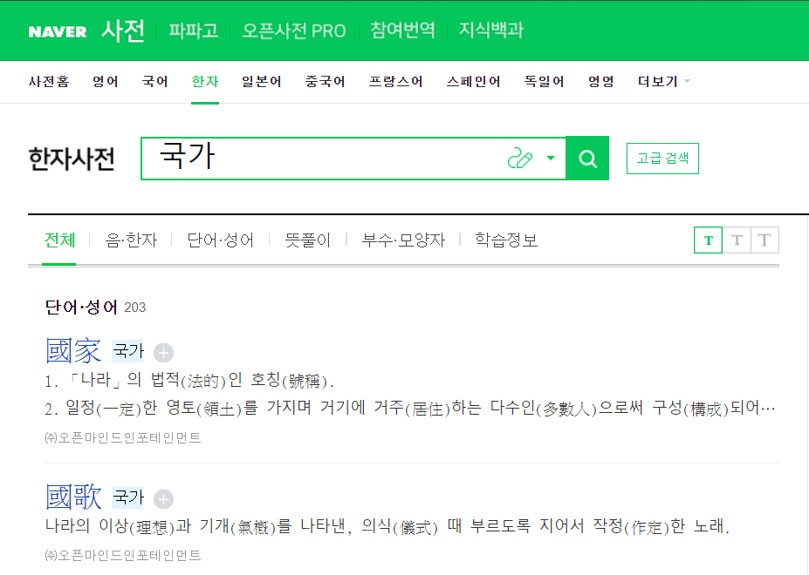
\includegraphics[width=\linewidth]{fig_2_1.jpg}
  \captionsetup{type=figure}
  \caption{The search results on the Naver Hanja Dictionary website interface}
  \label{fig:naver dictionary}
\end{figure}

%ch2.2
\section{Sentence-BERT}
Sentence-BERT\cite{reimers2019sentence} is a modification of the BERT model designed to produce semantically meaningful sentence embeddings. It utilizes siamese and triplet network structures to derive fixed-size vectors for sentences, which can be compared using cosine similarity. This makes Sentence-BERT particularly suitable for tasks such as sentence alignment and semantic search.
Sentence-BERT excels in sentence-pair regression tasks, such as semantic textual similarity (STS). In traditional BERT and RoBERTa\cite{liu2019roberta} models, both sentences need to be fed into the network, leading to significant computational overhead. In contrast, Sentence-BERT significantly reduces the computational effort, allowing for the identification of the most similar sentence pairs in seconds, whereas the same task would take hours with BERT or RoBERTa. Despite this reduction in computational time, Sentence-BERT maintains the high accuracy of the original BERT model.\\

%They concatenate the sentence embeddings u and v with the element-wise difference |u−v| . And multiply it with the trainable weight. The cosine similarity between the two sentence embeddings u and v is computed. For Triplet Objective Function, we give  an anchor sentence a, a positive sentence p, and a negative sentence n.
%And Triplet loss tunes the network. The distance between a and p is smaller than the distance between a and n. Margin ε ensures that Sp is at least closer to Sa than Sn.





%ch2.3
\section{BERT Model}
BERT (Bidirectional Encoder Representations from Transformers) is designed to pre-train deep bidirectional representations from unlabeled text.\cite{devlin2018bert} This framework allows the model to understand the context of a word based on its surrounding words in all directions (left and right). BERT's effectiveness is evaluated through two primary tasks: Masked Language Modeling (MLM) and Next Sentence Prediction (NSP).

\begin{itemize}
    \item \textbf{Masked Language Modeling (MLM):} In this task, some percentage of the input tokens are masked at random, and the objective is to predict the original vocabulary id of the masked word based only on its context. This helps the model to gain a deeper understanding of word relationships and context.
    \item \textbf{Next Sentence Prediction (NSP):} This task involves predicting whether a given sentence (Sentence B) is the subsequent sentence of another sentence (Sentence A). This aids the model in understanding the relationship between sentences, which is crucial for tasks like question answering and natural language inference.
\end{itemize}

BERT employs two primary strategies for utilizing its pre-trained representations:
\begin{itemize}
    \item \textbf{Feature-based Approach:} In this approach, the pre-trained BERT representations are used as features for downstream tasks, with minimal task-specific architecture modifications. This method leverages the rich embeddings from BERT without extensively modifying the original architecture.
    \item \textbf{Fine-tuning Approach:} Here, the pre-trained BERT model is fine-tuned on a specific task by adding an additional output layer. The entire model, including the pre-trained parameters, is trained jointly on the downstream task, allowing for task-specific adjustments while retaining the benefits of the pre-trained representations.
\end{itemize}

By leveraging these strategies, BERT achieves state-of-the-art results across a wide range of natural language processing tasks, demonstrating its versatility and powerful contextual understanding. For neural machine translation tasks, BERT can be used as the embedding layer of the model, providing rich contextual information that enhances translation accuracy. Figure 2.2 shows the framework of pre-training and fine-tuing for BERT model.

%fig 3.8
\begin{figure}[h!]
  \centering
  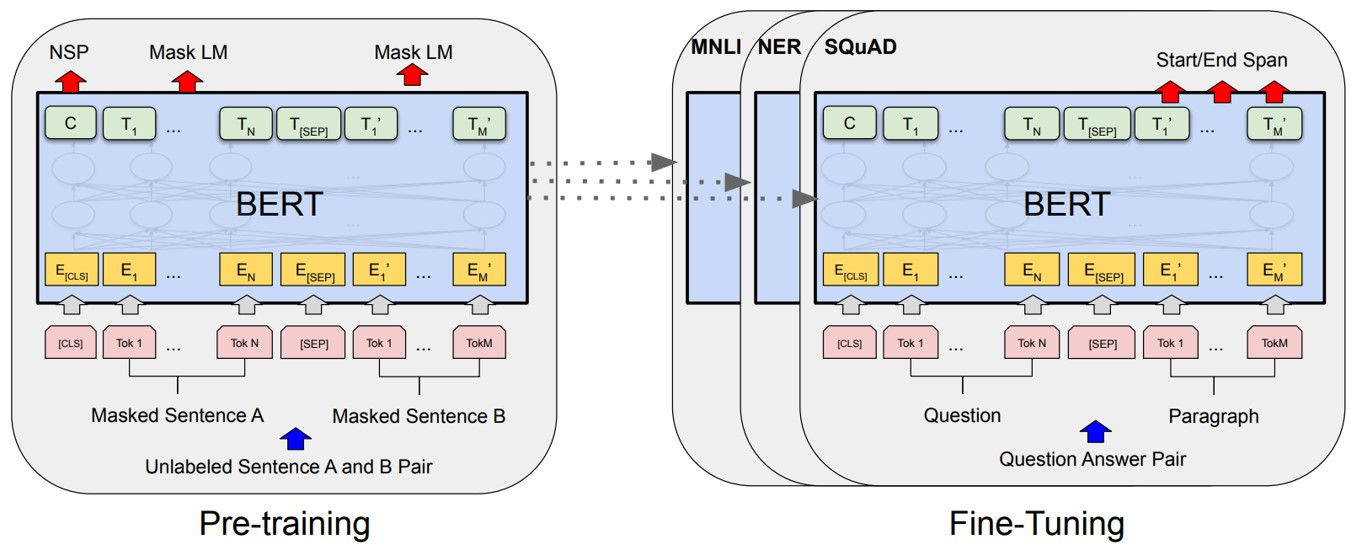
\includegraphics[width=\linewidth]{fig_3_bert.jpg}
  \captionsetup{type=figure}
  \caption{Framework of BERT model}
  \label{fig:framwork_bert}
\end{figure}

%ch2.3.1
\subsection{ckiplab/bert-base-chinese model}
The ckiplab/bert-base-chinese model is a BERT variant pre-trained on a large corpus of Chinese text, and it is available as an open-source model on Hugging Face.\cite{ckip-bert} This model is designed to understand the nuances of the Chinese language, including Traditional Chinese characters, making it a valuable resource for Chinese language processing tasks. The CKIP (Chinese Knowledge and Information Processing) group, formed in 1986 by the Institute of Information Science and the Institute of Linguistics of Academia Sinica, aims to establish a fundamental research environment for Chinese natural language processing.

The CKIP group's project provides a range of traditional Chinese transformer models, including ALBERT\cite{lan2019albert}, BERT, and GPT-2\cite{radford2019language}, as well as NLP tools such as word segmentation, part-of-speech tagging, and named entity recognition. Their language models are trained on the ZhWiki and CNA datasets\cite{10097977}. The tokenizer used in their models includes a total of 21,128 tokens.

%ch2.3.2
\subsection{Kim/bert-kor-base model}
The Kim/bert-kor-base\cite{kim2020lmkor} model is a BERT variant pre-trained on a large corpus of Korean text, available as an open-source model on Hugging Face. The data used for training this model includes 100 million major domestic commerce reviews and 20 million blog-type websites (75GB), Everyone's corpus (18GB), and Wikipedia and Namu Wiki (6GB). The training data is categorized into various fields such as cosmetics, food, electronics, and pets. The tokenizer for this model includes a total of 42,000 tokens.

%ch2.3.3
%\subsection{ChineseBERT: Chinese Pretraining Enhanced by Glyph and Pinyin Information}

%ch2.4
%\section{Transformer}

%ch3
\chapter{Methods}
%ch3.1
\section{Data Collection}
In this paper, given the scarcity of publicly available Traditional Chinese-Korean parallel sentence corpora, we utilize the Traditional Chinese and Korean versions of transcripts from the TED Talks website\cite{tedTalks} as our dataset. We employ web crawling to obtain these transcripts and use Sentence-BERT\cite{reimers2019sentence} to calculate the similarity between sentence pairs. By identifying highly similar sentence pairs, we construct our parallel sentence corpus.

%ch3.1.1
\subsection{Google Translation}
Googletrans library\cite{googletrans} is a free and unlimited Python library that implements the Google Translate API. We use Googletrans library to translate Traditional Chinese and Korean sentences to English as part of the sentence alignment process. Additionally, we use it to translate Traditional Chinese to Korean to obtain target sentences and then calculate the BLEU score as a benchmark.

We use Googletrans library to perform translations from Chinese to Korean, Chinese to English, and Korean to English. Figure 3.1 illustrates an example of a translation using Googletrans library.

%\setcounter{table}{2}
\begin{figure}[h!]
  \centering
  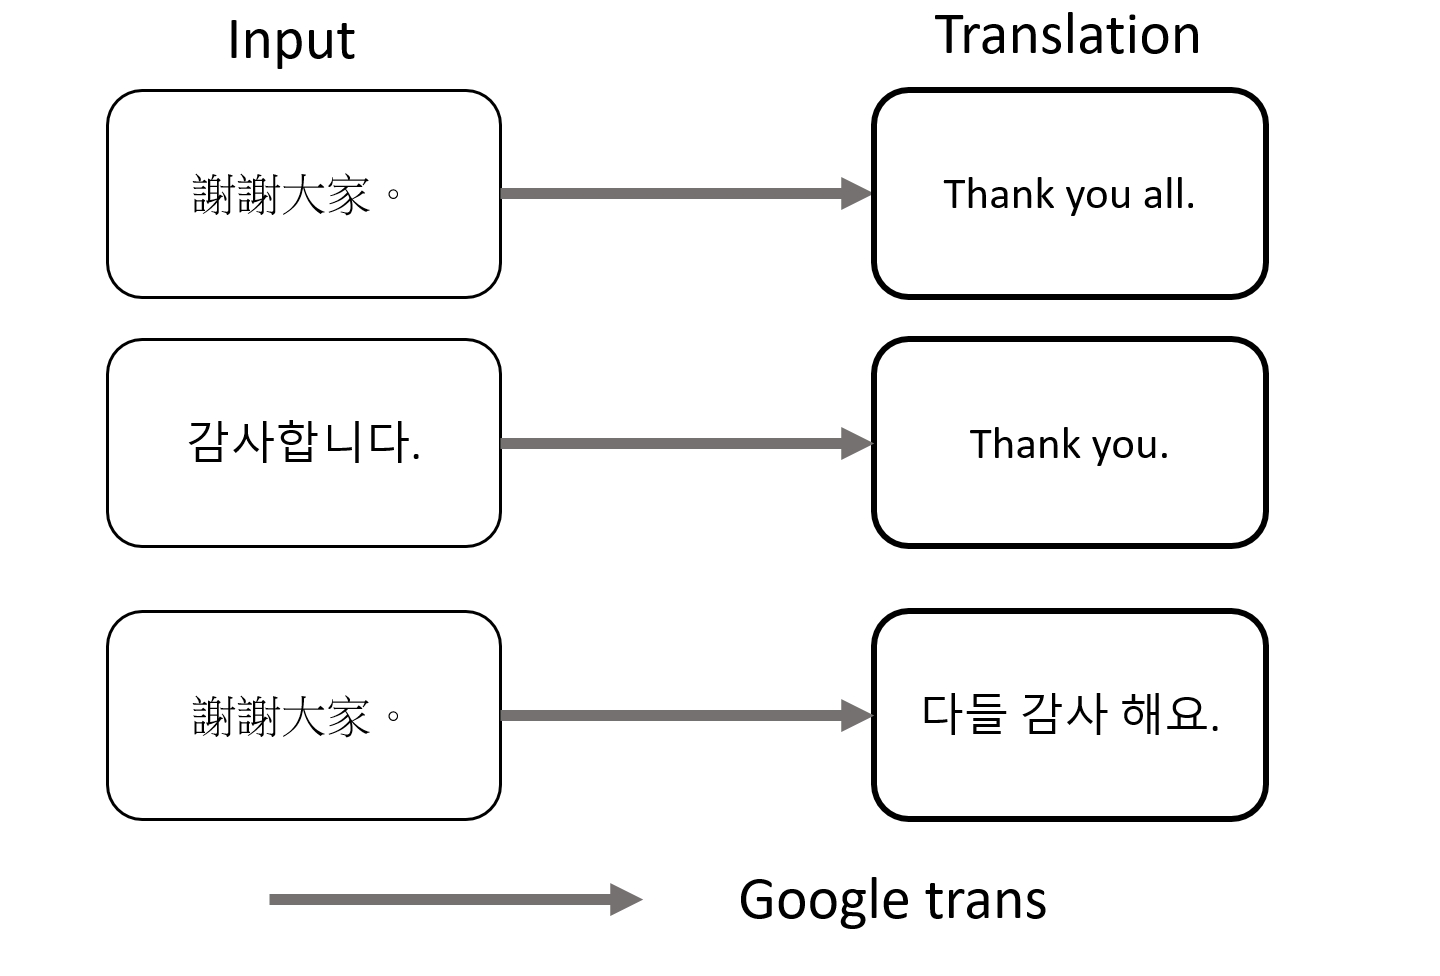
\includegraphics[width=\linewidth]{fig_3_1.jpg}
  \captionsetup{type=figure}
  \caption{Example of a translation using Googletrans library}
  \label{fig:googletrans}
\end{figure}

%ch3.1.2
\subsection{Web Crawling from TED Talks}
TED Talks feature a wide range of inspiring speeches covering various fields, including mental health, education, AI, business, communication, and more. In terms of subtitles, TED Talks offer numerous language translations, all provided by enthusiastic volunteers from around the world. These translations tend to be more colloquial and localized compared to professional translations.

For our study, we used Selenium to crawl the English, Korean, and Traditional Chinese transcripts from the TED Talks website to create our parallel sentence dataset. However, since the short sentences were not always aligned, we subsequently employed the Sentence-BERT method to find and align these short sentence pairs accurately.

We crawled a total of 4,937 transcripts from the TED Talks website.

Figure 3.2 illustrates an example of transcript timelines in different languages, highlighting the variations in timing and phrasing across translations.

%\setcounter{table}{2}
\begin{figure}[h!]
  \centering
  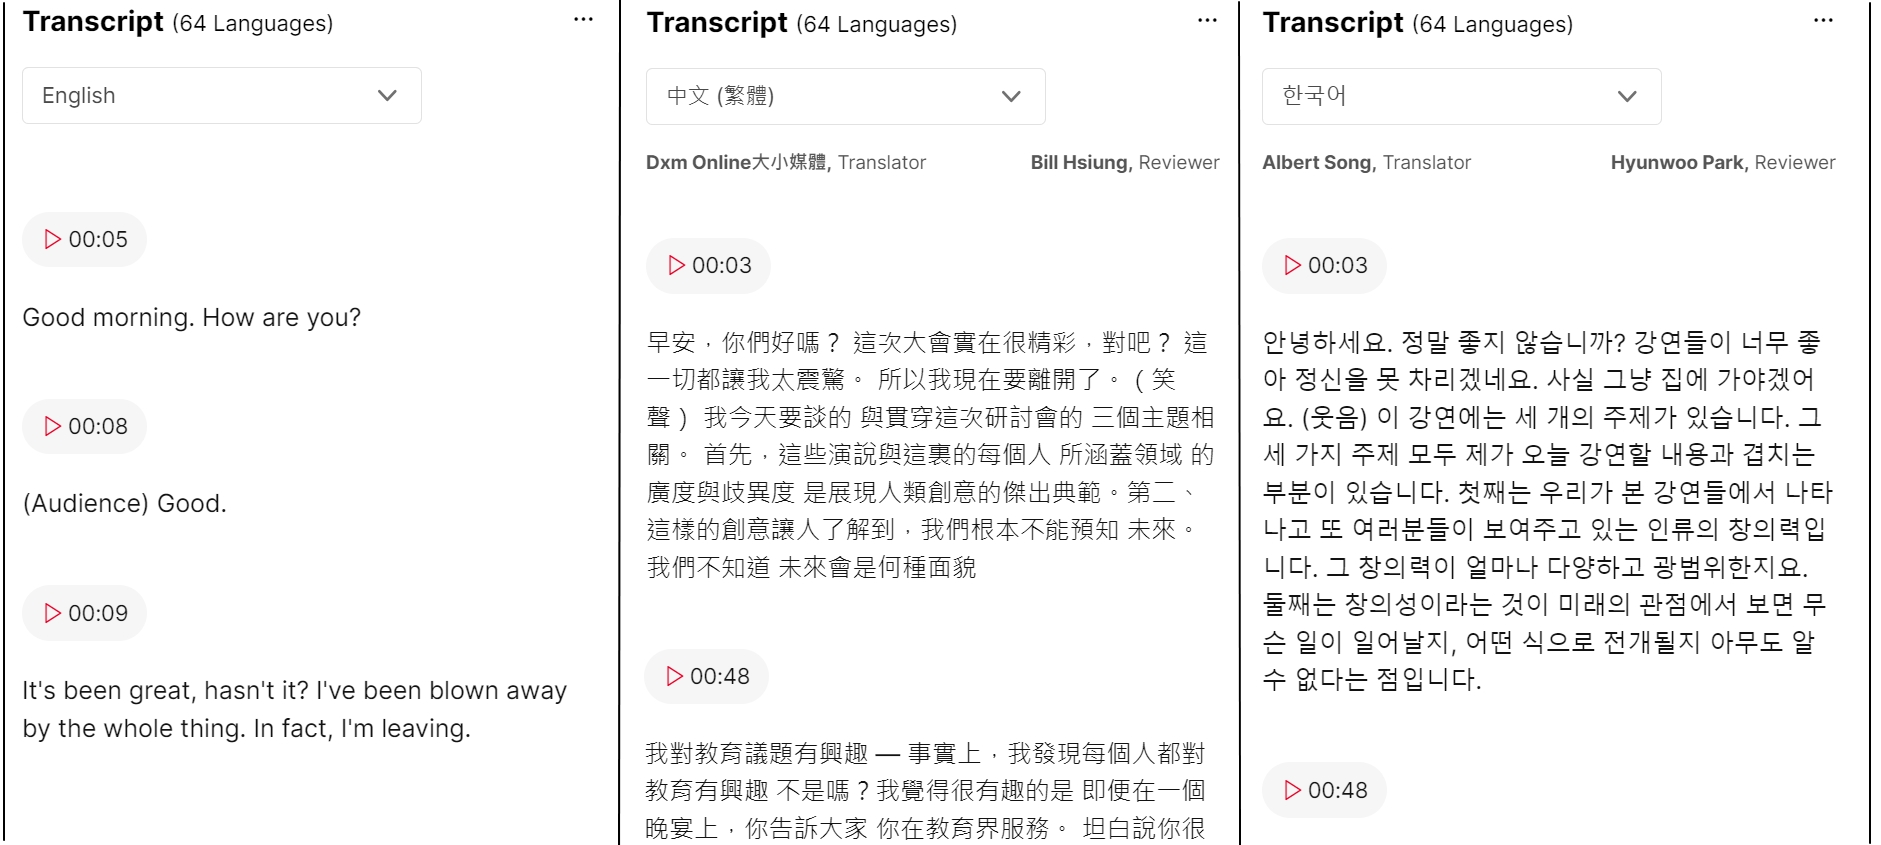
\includegraphics[width=\linewidth]{fig_3_2.jpg}
  \captionsetup{type=figure}
  \caption{Example of transcript timelines in different languages}
  \label{fig:transcript}
\end{figure}

%ch3.1.3
\subsection{Align Traditional Chinese - Korean sentence pairs with Sentence-BERT}
We use Sentence-BERT to evaluate the similarity between each sentence pair. Since Sentence-BERT is primarily trained on English texts, we first translate the Traditional Chinese and Korean sentences into English using Google Translate to improve similarity assessments. We then compare the translated Traditional Chinese and Korean sentences with the original English sentences.

We search for aligned sentence pairs in both forward and backward directions for each transcript. We retained sentence pairs with a similarity score greater than or equal to 0.5, ultimately preserving a total of 182,750 aligned sentences.

Figure 3.3 depicts the flowchart illustrating the alignment method utilizing Sentence-BERT. The flowchart visually outlines the steps involved in the alignment process, leveraging Sentence-BERT to establish correspondences between textual elements. This methodological diagram provides a clear overview of how Sentence-BERT is employed to enhance alignment accuracy and efficiency. Detailed steps and decision points within the flowchart elucidate the methodology, offering insights into the sequential processes employed for aligning textual data.

Figure 3.4 illustrates an example where the alignment method successfully identifies a parallel pair with high similarity. In contrast, Figure 3.5 presents an example where the alignment method fails to identify a parallel pair due to low similarity. These figures demonstrate the effectiveness and limitations of the alignment approach, highlighting scenarios where the method performs well and where it encounters challenges. By comparing these examples, we can better understand the factors influencing the alignment process and identify areas for potential improvement.

%\setcounter{table}{2}
\begin{figure}[h!]
  \centering
  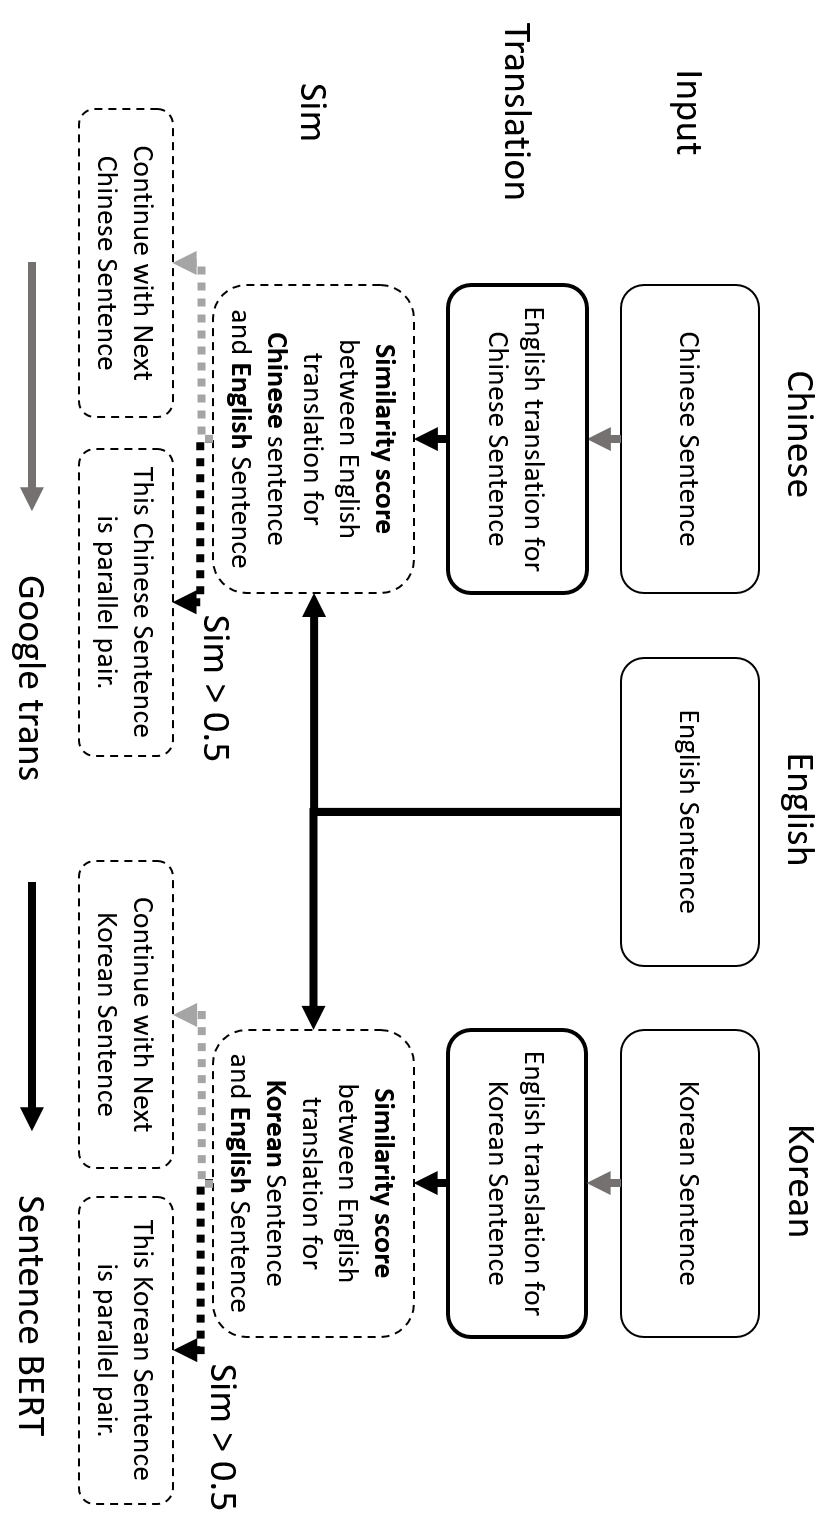
\includegraphics[width=0.75\linewidth]{fig_3_3.jpg}
  \captionsetup{type=figure}
  \caption{The flowchart of the alignment method utilizing Sentence-BERT}
  \label{fig:transcript}
\end{figure}

%\setcounter{table}{2}
\begin{figure}[h!]
  \centering
  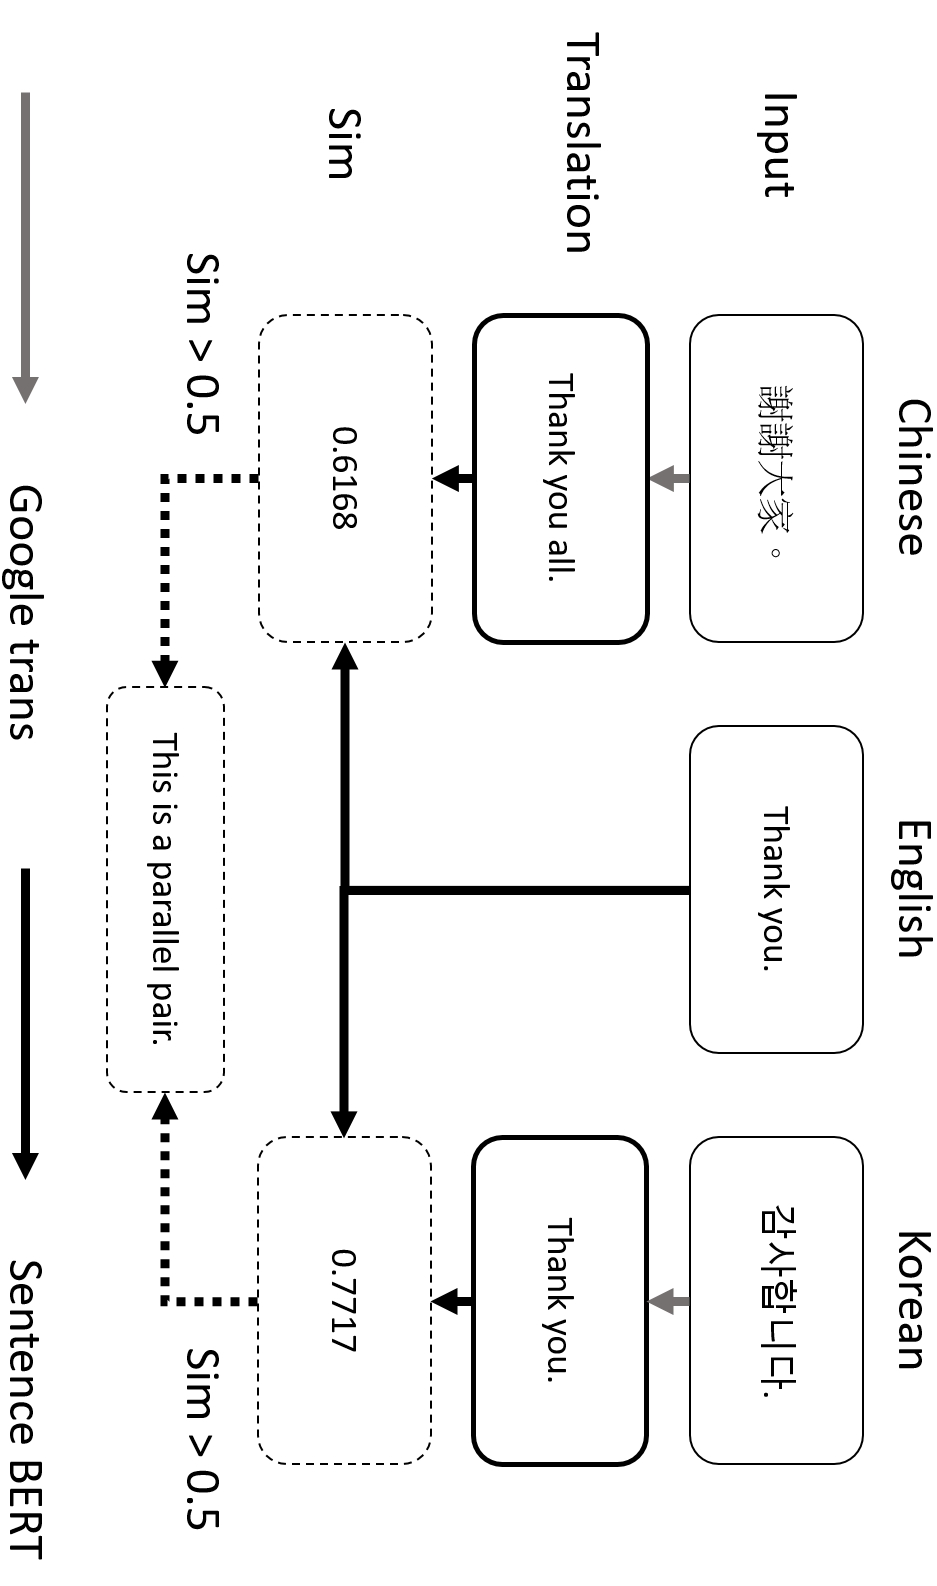
\includegraphics[width=0.75\linewidth]{fig_3_4.jpg}
  \captionsetup{type=figure}
  \caption{Successful example of the alignment method utilizing Sentence-BERT}
  \label{fig:transcript}
\end{figure}

%\setcounter{table}{2}
\begin{figure}[h!]
  \centering
  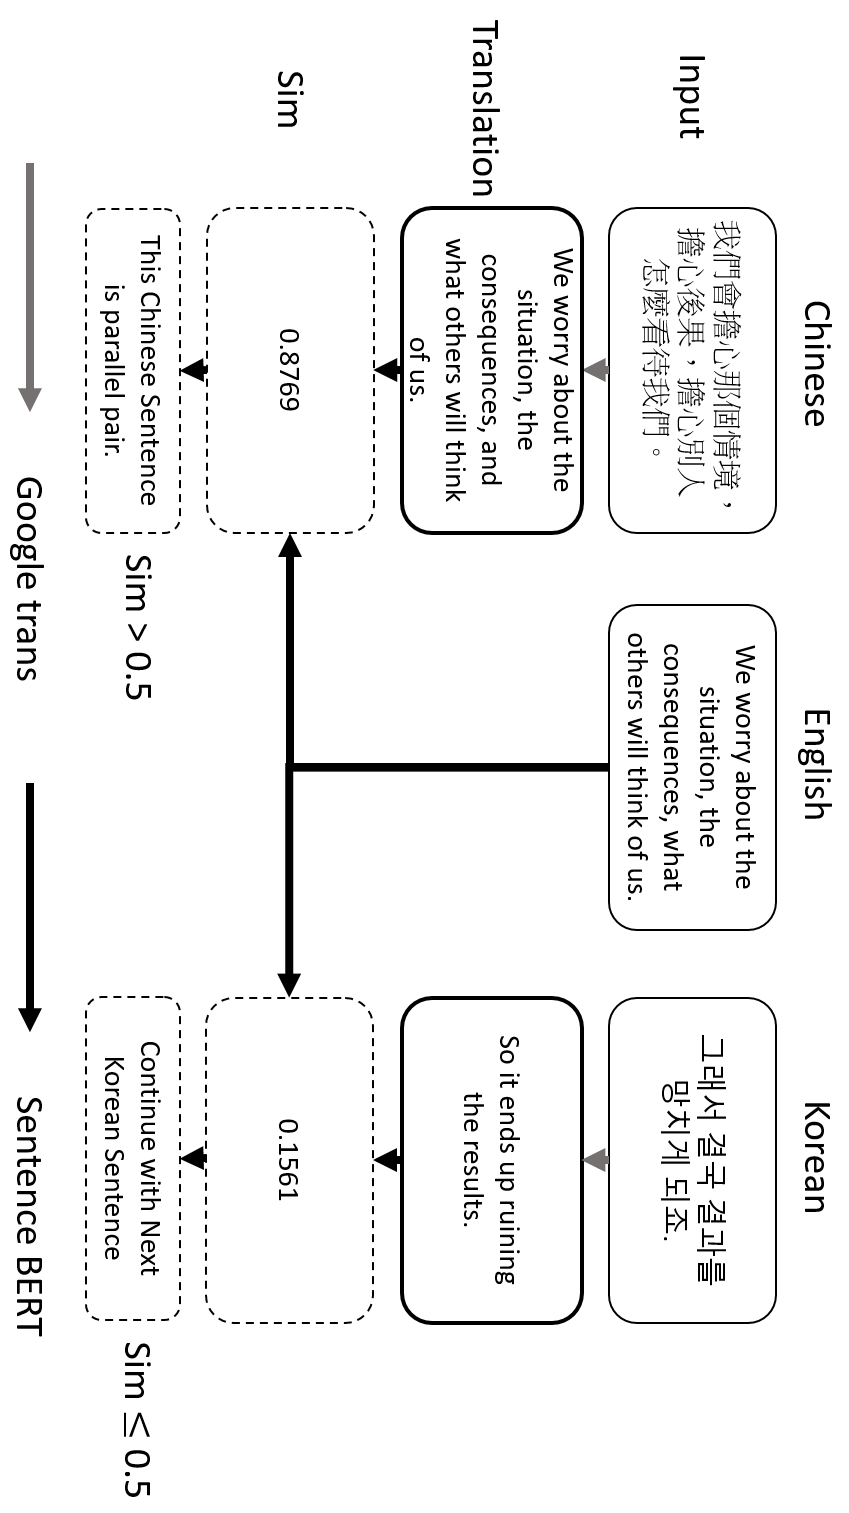
\includegraphics[width=0.75\linewidth]{fig_3_5.jpg}
  \captionsetup{type=figure}
  \caption{Failed example of the alignment method utilizing Sentence-BERT}
  \label{fig:transcript}
\end{figure}


%ch3.2
\section{Korean Hanja Data Collection}
Hangul originated from Chinese characters several centuries ago. After King Sejong invented Hangul, it gradually evolved into the modern Korean script. However, some aspects of Korean still retain the pronunciation of ancient Korean, which can be very similar to Chinese and Taiwanese. To utilize Hanja in representing Korean sentences, we use KoNLPy for word segmentation to identify all Korean pronunciation tokens that might correspond to Hanja. We then use a web crawler to obtain the Hanja groups corresponding to these Korean pronunciation tokens from the Naver Hanja Dictionary, creating a comprehensive Hanja  dictionary table.
Next, we use Sentence-BERT to calculate the similarity between the Korean sentence and the Chinese sentence after replacing the appropriate words with Hanja. We determine whether to replace the Korean words with their Hanja equivalents based on the difference in similarity scores. If the highest similarity score after replacement is greater than the original sentence's score by more than 0.001, we opt to make the substitution. This method ensures that the Hanja replacements meaningfully improve the alignment between Korean and Chinese sentences.

%ch3.2.1
\subsection{KoNLPy}
KoNLPy\cite{park2014konlpy} is a Python package designed for natural language processing (NLP) of the Korean language. We utilize KoNLPy to tokenize sentences in our dataset and extract all Korean word tokens. Subsequently, we use these tokens to retrieve their corresponding Hanja characters.
Table 3.1 displays Korean tokenized sentences processed using the KoNLPy library.

%tab 3.1
%\begin{figure}[h!]
%  \centering
%  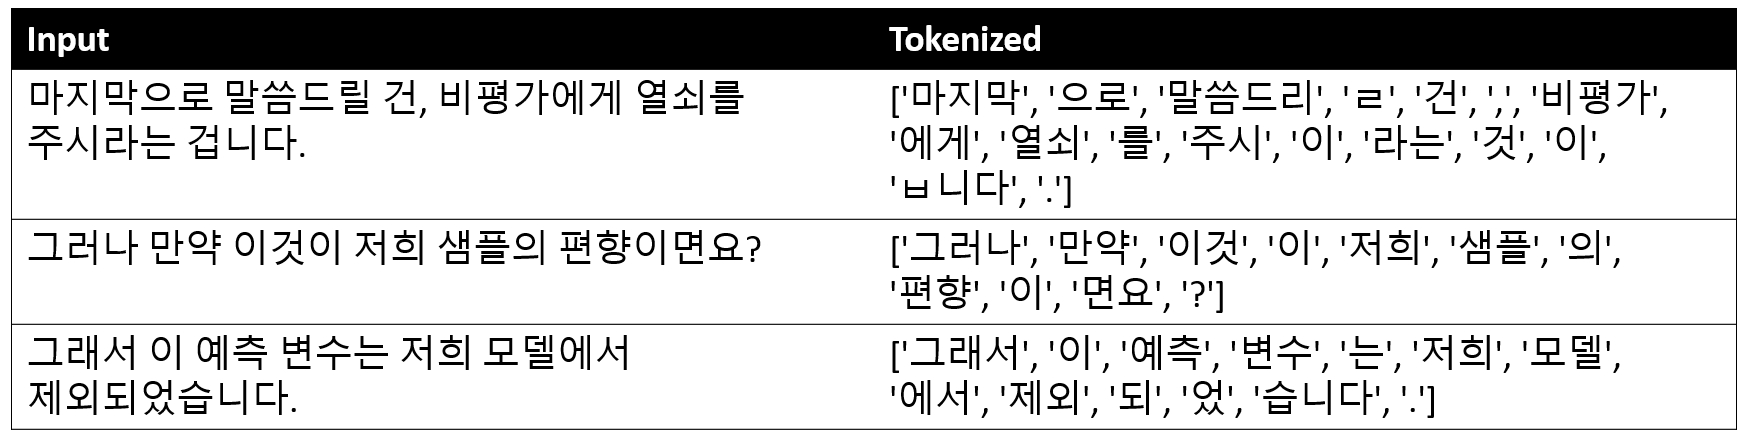
\includegraphics[width=\linewidth]{tab_3_konlpy.jpg}
%  \captionsetup{type=table}
%  \caption{Korean Tokenization using KoNLPy Library}
%  \label{fig:transcript}
%\end{figure}

\begin{table}
\begin{tabularx}{0.9\linewidth}{p{7cm} p{7cm}}
Input & Tokenized\\
\toprule
\krtext{마지막으로 말씀드릴 건, 비평가에게 열쇠를 주시라는 겁니다.} &  \krtext{['마지막', '으로', '말씀드리', 'ㄹ', '건', ',', '비평가', '에게', '열쇠', '를', '주시', '이', '라는', '것', '이', 'ㅂ니다', '.']} \\[.3ex]
\toprule
\krtext{그러나 만약 이것이 저희 샘플의 편향이면요?}  &  \krtext{['그러나', '만약', '이것', '이', '저희', '샘플', '의', '편향', '이', '면요', '?']} \\[.3ex]
\toprule
\krtext{그래서 이 예측 변수는 저희 모델에서 제외되었습니다.}  & \krtext{['그래서', '이', '예측', '변수', '는', '저희', '모델', '에서', '제외', '되', '었', '습니다', '.']} \\
\bottomrule
\end{tabularx}
\caption{Korean Tokenization using KoNLPy Library}
\label{tab:notation}
\end{table}

%ch3.2.2
\subsection{Web Crawling from Naver Dictionary}
We utilize the Hanja Dictionary from Naver Dictionary to find the corresponding Hanja characters for Korean tokens.\cite{NaverDictionary} Using Selenium, we perform dynamic web crawling to search the Naver Hanja Dictionary and verify whether each Korean token has a corresponding Hanja character. If a match is found and the number of characters is the same, it is stored in our Hanja dictionary table.  Table 3.2 presents some examples of Hangul to Hanja pairs, which were obtained by crawling data from the Naver Hanja Dictionary website.

%tab 3.2
%\begin{figure}[h!]
%  \centering
%  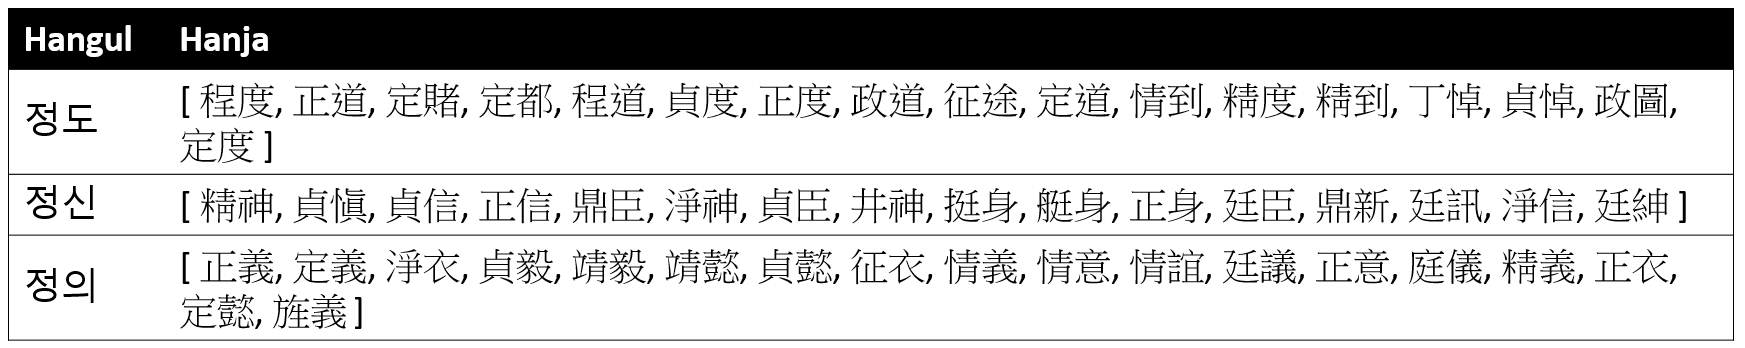
\includegraphics[width=\linewidth]{tab_3_hanja.jpg}
%  \captionsetup{type=table}
%  \caption{Examples in the Hanja Dictionary Table }
%  \label{fig:transcript}
%\end{figure}

\begin{table}
\begin{tabularx}{0.9\linewidth}{p{3cm} p{7cm}}
Hangul & Hanja \\
\toprule
\krtext{정도} &  [ 程度, 正道, 定賭, 定都, 程道, 貞度, 正度, 政道, 征途, 定道, 情到, 精度, 精到, 丁悼, 貞悼, 政圖, 定度 ] \\[.3ex]
\toprule
\krtext{정신}  &  [ 精神, 貞愼, 貞信, 正信, 鼎臣, 淨神, 貞臣, 井神, 挺身, 艇身, 正身, 廷臣, 鼎新, 廷訊, 淨信, 廷紳 ]  \\[.3ex]
\toprule
\krtext{정의}  & [ 正義, 定義, 淨衣, 貞毅, 靖毅, 靖懿, 貞懿, 征衣, 情義, 情意, 情誼, 廷議, 正意, 庭儀, 精義, 正衣, 定懿, 旌義 ] \\
\bottomrule
\end{tabularx}
\caption{Examples in the Hanja Dictionary Table}
\label{tab:notation}
\end{table}

Through this process, we obtained a total of 23,151 Korean tokens and 56,795 corresponding Chinese characters, creating a comprehensive resource for our translation tasks.


%ch3.2.3
\subsection{Transform Korean Sentence to Hanja Sentence with Sentence-BERT}
First, we use the KoNLPy tokenizer to extract tokens from Korean sentences. Next, we identify tokens that are present both in the sentence and in our Hanja dictionary table, which we built through web scraping from the Naver Hanja Dictionary website.

Second, we sequentially transform the Korean tokens into all corresponding Hanja characters found in the Hanja dictionary table. Using Sentence-BERT, we then determine the most similar Hanja sentence compared to the original Korean sentence.

Finally, to find the Hanja that best matches the semantic meaning of the Korean token in the original Korean sentence, we compare the Korean sentence integrated with Hanja to the Chinese sentence. We use Sentence-BERT to calculate the similarity score between the Chinese sentence and the Korean sentence with merged Hanja. We retain the Hanja sentence with the highest cosine similarity score among all possible Hanja sentences. If the similarity score between the transformed Hanja sentence and the Chinese sentence exceeds that of the original Korean sentence by more than 0.001, we preserve the Hanja sentence for further processing.

Figure 3.6 illustrates the flowchart for identifying the most suitable Hanja characters from a Korean sentence. This process involves using a Hanja dictionary table and the Sentence-BERT method to evaluate the similarity between Hangul and Hanja. The flowchart outlines each step of the alignment method, demonstrating how Sentence-BERT enhances the accuracy of matching Hangul text with its corresponding Hanja characters. 
Figure 3.7 demonstrates the process of selecting the most suitable Hanja for a given Korean word using our method. 
Figure 3.8 illustrates the extraction of Hanja sentences from Korean sentences using this approach. These figures exemplify how Sentence-BERT is applied to evaluate the similarity between Hangul and Hanja, thereby facilitating accurate Hanja selection and sentence formation.

\clearpage
\begin{figure}[h!]
  \centering
  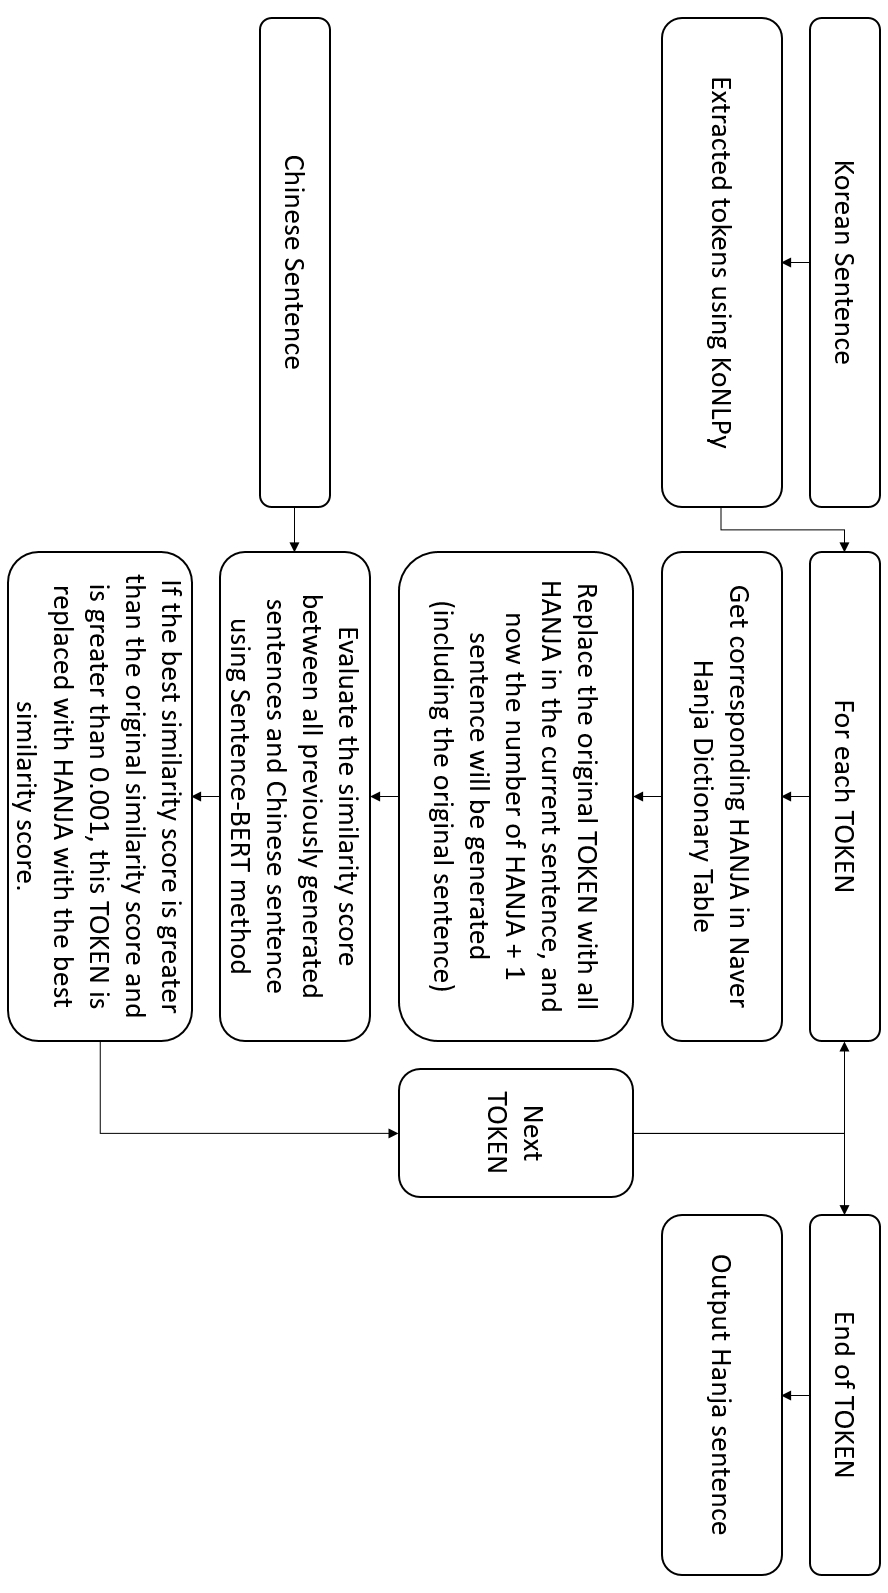
\includegraphics[width=0.75\linewidth]{fig_3_6.jpg}
  \captionsetup{type=figure}
  \caption{Flowchart for identifying the most suitable Hanja characters from a Korean sentence}
  \label{fig:flowchar_hanja}
\end{figure}


\clearpage
\begin{figure}[h!]
  \centering
  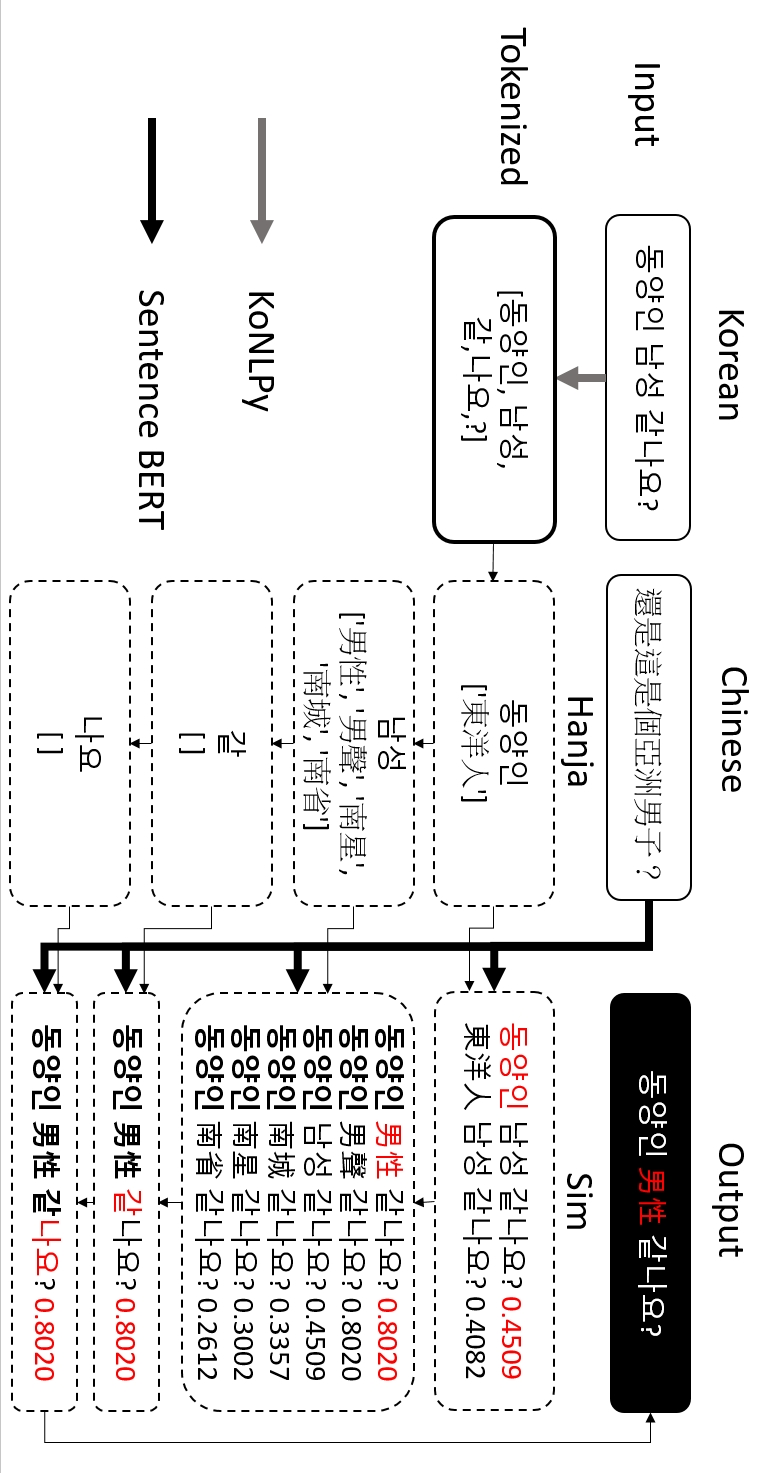
\includegraphics[width=0.75\linewidth]{fig_3_7.jpg}
  \captionsetup{type=figure}
  \caption{Process of selecting the most suitable Hanja for a given Korean word}
  \label{fig:example_hanja_process}
\end{figure}


\clearpage
%tab3.3
\begin{figure}[h!]
  \centering
  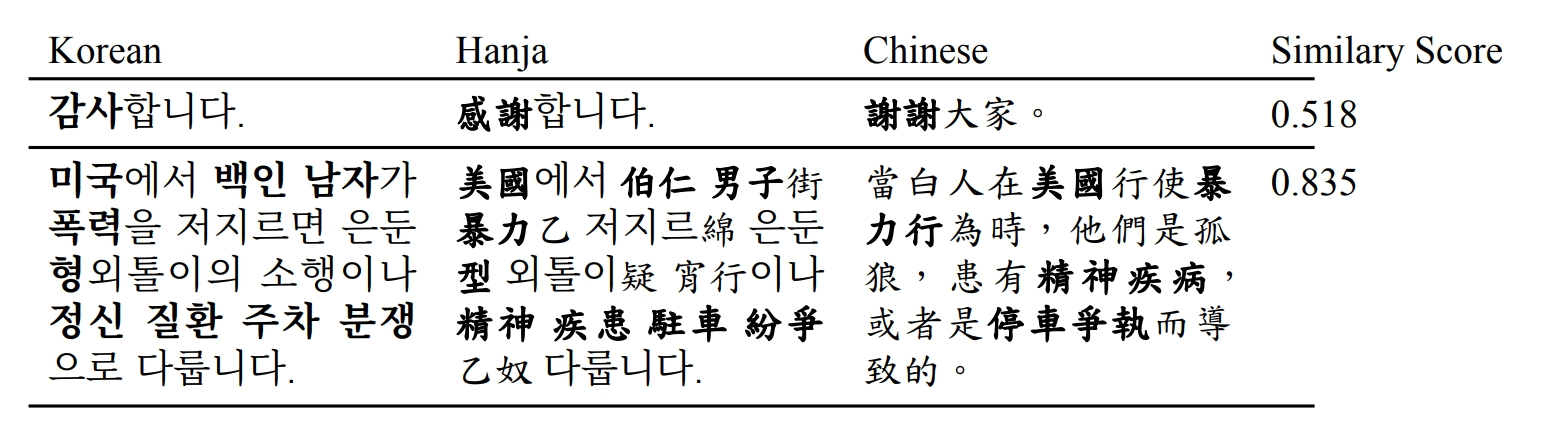
\includegraphics[width=\linewidth]{tab_3_3.jpg}
  \captionsetup{type=table}
  \caption{Extraction of Hanja sentences from Korean sentences using our approach}
  \label{fig:example_hanja_sentences}
\end{figure}

%\begin{table}
%\begin{tabularx}{0.9\linewidth}{p{4cm} p{4cm} p{4cm} p{4cm}}
%Korean & Hanja & Chinese & Similary Score \\
%\toprule
%\krtext{\textbf{감사}합니다.}
%& \textbf{感謝}\krtext{합니다.}
%& \textbf{謝謝}大家。
%& 0.518 \\[.3ex]
%\toprule
%\krtext{\textbf{미국}에서 \textbf{백인 남자}가 \textbf{폭력}을 저지르면 은둔 \textbf{형} 외톨이의 소행이나 \textbf{정신 질환 주차 분쟁}으로 다룹니다.}
%&  \textbf{美國}\krtext{에서} \textbf{伯仁} \textbf{男子}街 \textbf{暴力}乙 \krtext{저지르}綿 \krtext{은둔} \textbf{型} \krtext{외톨이}疑 宵行\krtext{이나} \textbf{精神 疾患 駐車 紛爭}乙奴 \krtext{다룹니다.} 
%& 當白人在\textbf{美國}行使\textbf{暴力行}為時,他們是孤狼,患有\textbf{精神疾病},或者是\textbf{停車爭執}而導致的。
%& 0.835 \\[.3ex]
%\bottomrule
%\end{tabularx}
%\caption{Extraction of Hanja sentences from Korean sentences using our approach}
%\label{tab:notation}
%\end{table}


%ch3.3
\section{Phonetic Data Extraction}
Phonetic notation helps disambiguate homophones and aids in pronunciation, enhancing the translation model's understanding of both languages. In this paper, we use Dragonmapper's  "\textbf{\textit{hanzi.to\_zhuyin(chinese sentence)}}"  function to convert Chinese characters into Bopomofo. This allows us to extract the phonetic representation of Chinese sentences , which is crucial for aligning them with Korean sentences. By incorporating phonetic data, we can improve the model's ability to capture subtle nuances in pronunciation and meaning, ultimately leading to more accurate translations.

%ch3.3.1
\subsection{Dragon Mapper}
Dragonmapper\cite{dragonMapper} is a Python library designed for working with Chinese text, particularly for tasks involving phonetic transcription and pronunciation. It provides tools for converting Chinese characters into Bopomofo. Additionally, Dragonmapper can be used to analyze and process Chinese text, making it useful for various natural language processing (NLP) applications.

In this paper, we use Dragonmapper to extract phonetic data from Chinese text. By converting Traditional Chinese characters into their corresponding Bopomofo, we can better understand the pronunciation and phonetic structure of the text. This is particularly useful for aligning Chinese sentences with Korean sentences, as phonetic similarities can play a significant role in achieving accurate translation.

The results of the extractions from Chinese sentences are shown in Table 3.1. We will incorporate these extractions into our tokenizer to enhance performance. By adding phonetic data obtained through Dragonmapper, we aim to improve the model's ability to handle pronunciation and homophones, thus providing more accurate and contextually appropriate translations.

%tab3.4
\begin{figure}[h!]
  \centering
  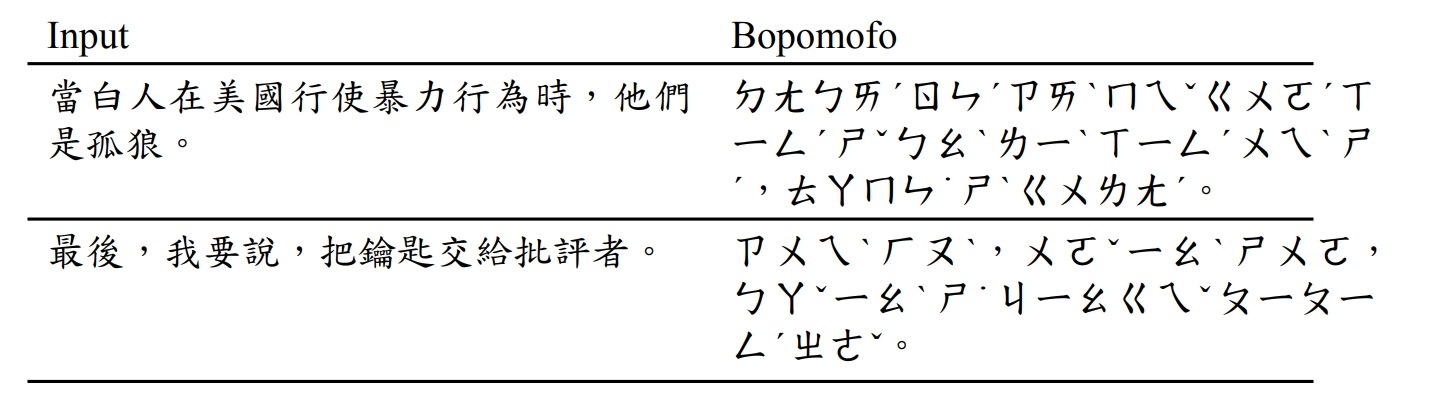
\includegraphics[width=\linewidth]{tab_3_4.jpg}
  \captionsetup{type=table}
  \caption{The results of the extractions from Chinese sentences using Dragon Mapper}
  \label{tab:dragonmapper}
\end{figure}

%\begin{table}
%\begin{tabularx}{0.9\linewidth}{p{7cm} p{7cm}}
%Input & Bopomofo\\
%\toprule
%當白人在美國行使暴力行為時,他們是孤狼。 
%& ㄉㄤㄅㄞˊㄖㄣˊㄗㄞˋㄇㄟˇㄍㄨㄛˊㄒㄧㄥˊㄕˇㄅㄠˋㄌㄧˋㄒㄧㄥˊㄨㄟˋㄕˊ,ㄊㄚㄇㄣ˙ㄕˋㄍㄨㄌㄤˊ。\\
%\toprule
%最後,我要說,把鑰匙交給批評者。 
%&  ㄗㄨㄟˋㄏㄡˋ,ㄨㄛˇㄧㄠˋㄕㄨㄛ,ㄅㄚˇㄧㄠˋㄕ˙ㄐㄧㄠㄍㄟˇㄆㄧㄆㄧㄥˊㄓㄜˇ。\\
%\bottomrule
%\end{tabularx}
%\caption{The results of the extractions from Chinese sentences using Dragon Mapper}
%\label{tab:notation}
%\end{table}

%ch3.4
\section{Tokenization}
In this paper, we primarily utilize tokenizers developed by the HuggingFace team for the tokenization process. Specifically, we employ the 'Bert-base-chinese' tokenizer for Chinese text and the 'Kim/bert-kor-base' tokenizer for Korean text. Additionally, we incorporate supplementary phonetic tokens for Bopomofo to enhance the tokenization accuracy for Chinese.

%ch3.4.1
\subsection{HuggingFace Tokenizers}
We use a tokenizer to split the input into subwords and transform these subwords into IDs as input for our training model. Tokenizers accomplish several tasks:

\begin{itemize}
    \item \textbf{Tokenization}: Splitting a string into subword tokens, converting these tokens to IDs and back, and performing encoding and decoding by tokenizing and converting text to integers.
    \item \textbf{Vocabulary Management}: Adding new tokens to the vocabulary independently of the underlying structure.
    \item \textbf{Special Tags Handling}: Managing special tokens like \texttt{[BOS]}, \texttt{[MASK]}, etc., by adding them, assigning properties in the token generator for easy access, and ensuring they are not split during tokenization.
\end{itemize}

In our approach, we primarily use the \texttt{Bert-base-chinese} tokenizer. We also incorporate additional tokens for Korean and Bopomofo to enhance the tokenization process.


%ch3.4.2
\subsection{Add Korean and Bopomofo Tokens}
We augment our tokenizer with additional tokens for Korean Hangul and Bopomofo (phonetic annotations for Chinese). This enhancement ensures that our model can effectively handle these additional linguistic features. We use the \texttt{Bert-base-chinese} tokenizer as the base tokenizer, integrating Hangul tokens from the \texttt{Kim/bert-kor-base} tokenizer for Korean, and adding Bopomofo tokens from all phonetic combinations.

The \texttt{Bert-base-chinese} tokenizer contains 21,128 tokens, the Bopomofo tokens add up to 2,089, and the \texttt{Kim/bert-kor-base} tokenizer includes 42,000 tokens. After merging all tokens, we obtain a total of 63,662 tokens. 

Table 3.4 presents the token counts for each tokenizer before and after merging.

%tab3.5
%\begin{figure}[h!]
%  \centering
%  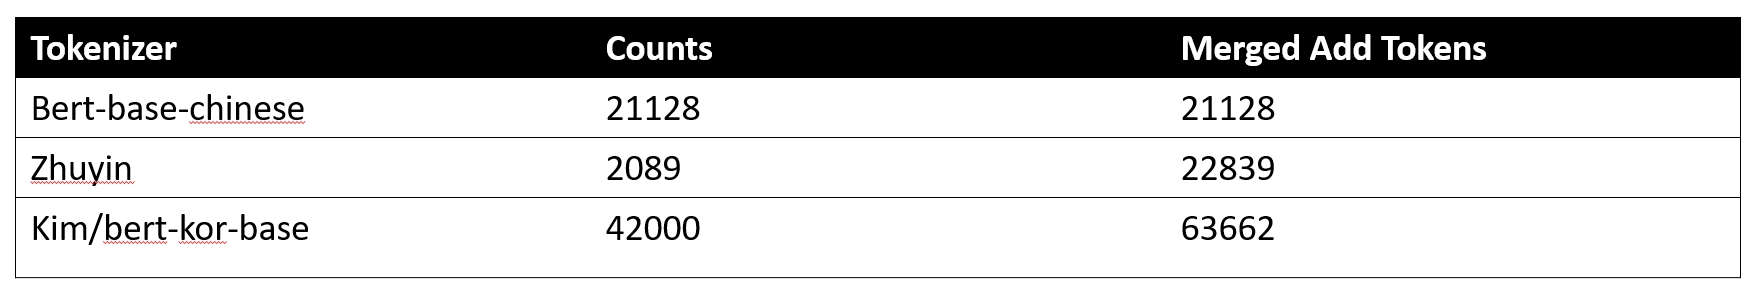
\includegraphics[width=\linewidth]{tab_3_number_of_tokens.jpg}
%  \captionsetup{type=table}
%  \caption{Counts of tokens in Tokenizers}
%  \label{tab:token_counts}
%\end{figure}

\begin{table}
\begin{tabularx}{0.9\linewidth}{p{4cm} p{4cm} p{4cm}}
Tokenizer
& Counts
& Merged Add Tokens
\\
\toprule
Bert-base-chinese
& 21128
& 21128
\\
Bopomofo
&  2089
& 22839\\
Kim/bert-kor-base
& 42000
& 63662\\
\bottomrule
\end{tabularx}
\caption{Counts of tokens in Tokenizers}
\label{tab:notation}
\end{table}

%ch3.4.3
\subsection{Comparison of Tokenizers}
We compare different tokenization approaches, including the initial \texttt{Bert-base-chinese} tokenizer and the augmented version with additional Korean and Bopomofo tokens. The initial \texttt{Bert-base-chinese} tokenizer cannot identify Korean Hangul and Bopomofo tokens. However, after incorporating these additional tokens, the tokenizer can successfully recognize non-Chinese characters, including Korean Hangul and Bopomofo.

Table 3.5 presents the different tokenization results between using the initial tokenizer and the augmented tokenizer with Korean and Bopomofo tokens.

%tab3.6
\begin{figure}[h!]
  \centering
  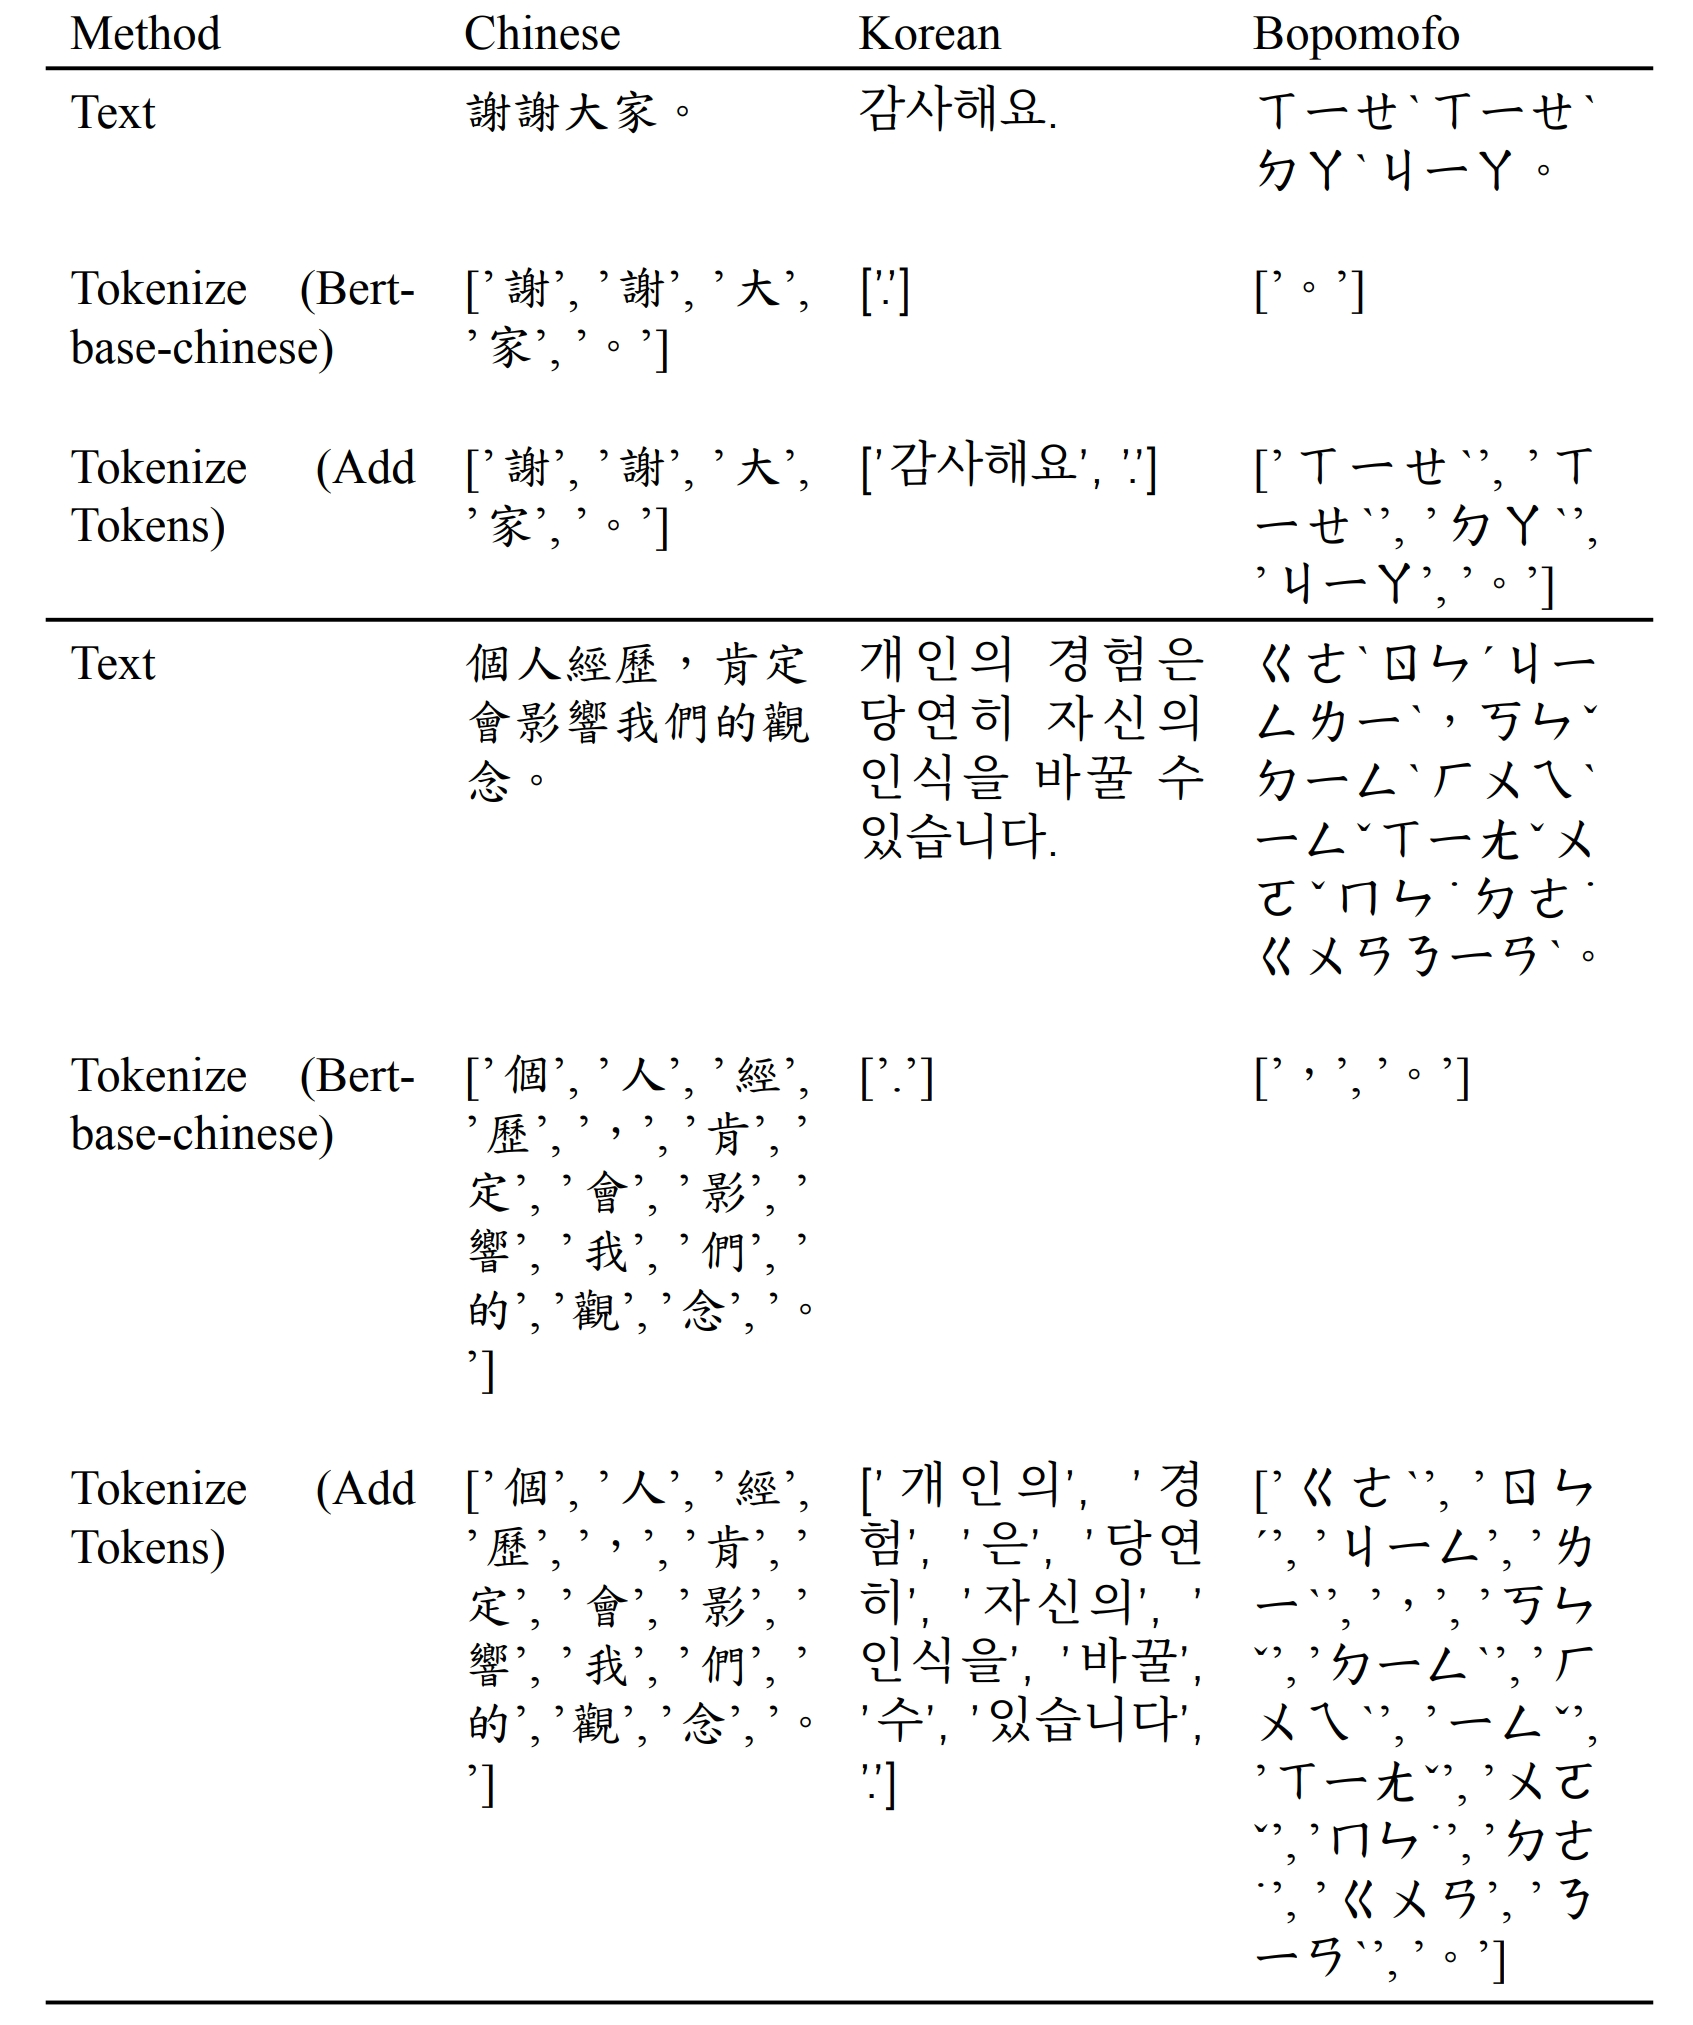
\includegraphics[width=\linewidth]{tab_3_6.jpg}
  \captionsetup{type=table}
  \caption{Comparison of Tokenizers}
  \label{tab:compare_of_tokenizer}
\end{figure}


%\begin{table}
%\begin{tabularx}{0.9\linewidth}{p{3cm} p{3cm} p{3cm} p{3cm}}
%Method
%& Chinese
%& Korean
%& Bopomofo
%\\
%\toprule
%Text
%& 謝謝大家。
%& \krtext{감사해요.}
%& ㄒㄧㄝˋㄒㄧㄝˋㄉㄚˋㄐㄧㄚ。\\
%\\
%Tokenize
%(Bert-base-chinese)
%&  ['謝', '謝', 
%'大', '家', '。']
%& \krtext{['.']}
%& ['。']\\
%\\
%Tokenize
%(Add Tokens)
%& ['謝', '謝', 
%'大', '家', '。']
%& \krtext{['감사해요', '.']}
%& ['ㄒㄧㄝˋ', 'ㄒㄧㄝˋ', 'ㄉㄚˋ', 'ㄐㄧㄚ', '。']\\
%\toprule
%Text
%& 個人經歷,肯定會影響我們的觀念。
%& \krtext{개인의 경험은 당연히 자신의 인식을 바꿀 수 있습니다.}
%& ㄍㄜˋㄖㄣˊㄐㄧㄥㄌㄧˋ,ㄎㄣˇㄉㄧㄥˋㄏㄨㄟˋㄧㄥˇㄒㄧㄤˇㄨㄛˇㄇㄣ˙ㄉㄜ˙ㄍㄨㄢㄋㄧㄢˋ。\\
%\\
%Tokenize   
%(Bert-base-chinese)
%&  ['個', '人', '經', '歷', ',', '肯', '定', '會', '影', '響', '我', '們', '的', '觀', '念', '。']
%& ['.']
%& [',', '。']\\
%\\
%Tokenize   
%(Add Tokens)
%& ['個', '人', '經', '歷', ',', '肯', '定', '會', '影', '響', '我', '們', '的', '觀', '念', '。']
%& \krtext{['개인의', '경험', '은', '당연히', '자신의', '인식을', '바꿀', '수', '있습니다', '.']}
%& ['ㄍㄜˋ', 'ㄖㄣˊ', 'ㄐㄧㄥ', 'ㄌㄧˋ', ',', 'ㄎㄣˇ', 'ㄉㄧㄥˋ', 'ㄏㄨㄟˋ', 'ㄧㄥˇ', 'ㄒㄧㄤˇ', 'ㄨㄛˇ', 'ㄇㄣ˙', 'ㄉㄜ˙', 'ㄍㄨㄢ', 'ㄋㄧㄢˋ', '。']\\
%\bottomrule
%\end{tabularx}
%\caption{Comparison of Tokenizers}
%\label{tab:notation}
%\end{table}

%ch3.5
\section{Embedding}
Embedding layers are crucial for converting tokens into dense vector representations that capture their semantic meaning. We use BERT to extract the last hidden state as the embedding of the input sentence. Specifically, we utilize the \texttt{ckiplab/bert-base-chinese} BERT model developed by the CKIP team. This model is trained for Traditional Chinese, providing robust and accurate embeddings for our tasks.

%ch3.5.1
\subsection{BERT}
BERT (Bidirectional Encoder Representations from Transformers) is a pre-trained language model developed by Google that has significantly advanced natural language processing tasks. The BERT model leverages a transformer architecture to learn deep bidirectional representations by jointly conditioning on both left and right context in all layers.

Embedding layers in BERT are crucial for converting tokens into dense vector representations that capture their semantic meaning. In BERT, the input tokens are first converted into embeddings through a combination of three embeddings:

\begin{itemize}
    \item \textbf{Token Embeddings}: Represent the individual tokens (words or subwords) in the input text.
    \item \textbf{Segment Embeddings}: Distinguish between different sentences in tasks where sentence pairs are involved (e.g., question-answering).
    \item \textbf{Position Embeddings}: Encode the position of each token in the input sequence to preserve the order of words.
\end{itemize}

These embeddings are summed together to form the final input embeddings, which are then fed into the transformer layers of BERT.

For our work, we use BERT to extract the last hidden state as the embedding of the input sentence. Specifically, we utilize the \texttt{ckiplab/bert-base-chinese} BERT model developed by the CKIP team. This model is trained on Traditional Chinese text, providing robust and accurate embeddings for tasks involving Traditional Chinese.

By leveraging BERT's embeddings, we can capture rich contextual information and semantic meaning from the input text, which significantly enhances the performance of our downstream natural language processing tasks.
Figure 3.8 shows the input embeddings for BERT model.

%fig 3.8
\begin{figure}[h!]
  \centering
  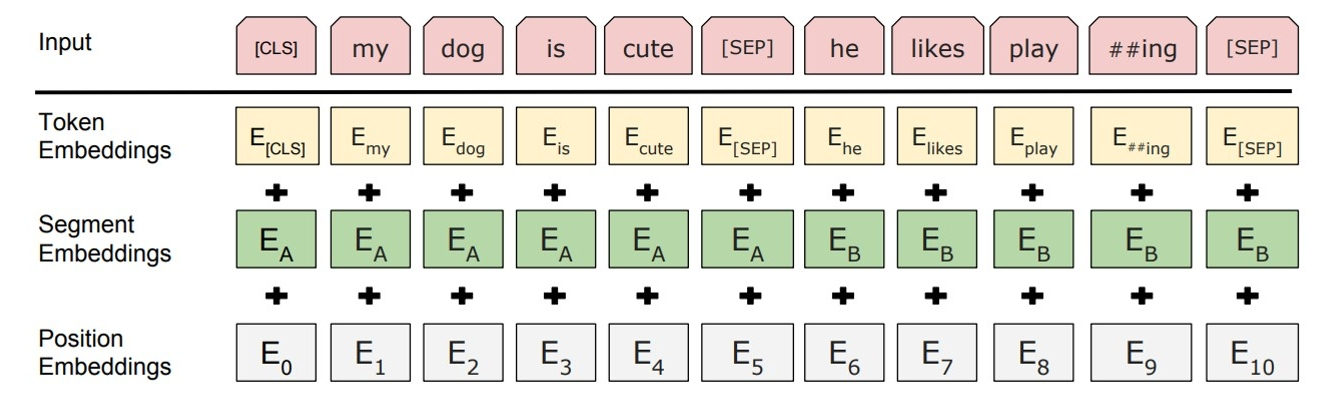
\includegraphics[width=\linewidth]{fig_3_bert_presentation.jpg}
  \captionsetup{type=figure}
  \caption{BERT input presentation}
  \label{fig:bert_presentation}
\end{figure}


%ch3.5.2
\subsection{Joint Embedding}
Joint embedding is a technique that projects words from different languages or modalities into a shared embedding space. This approach allows for capturing the semantic relationships between words more effectively. Meta-embedding\cite{kiela-etal-2018-dynamic}, a specific form of joint embedding, involves combining multiple embeddings to create a single, unified representation. This is particularly useful in scenarios where multiple sources of information, such as different scripts or phonetic annotations, need to be integrated.

In this paper, we utilize meta-embedding to merge embeddings from three different sources: Chinese characters, Korean Hanja characters, and Bopomofo (a phonetic notation system used for Traditional Chinese). By combining these embeddings, we aim to enrich the semantic representation and improve the translation performance between Traditional Chinese and Korean. Specifically, we use a ratio of 0.5:0.25:0.25 to merge Chinese, Hanja, and Bopomofo embeddings respectively. This ratio is chosen to balance the influence of each component, ensuring that the primary script (Chinese characters) has the most significant impact while still incorporating the additional contextual information provided by Hanja and Bopomofo.

%ch3.6
\section{Model}

%ch3.6.1
\subsection{Framework}
In the paper by Jinhua Zhu (2020)\cite{zhu2020incorporating}, a BERT-fused model is proposed, which leverages the representation from BERT by integrating it into all layers of the model rather than using it solely as input embeddings. This approach resulted in improved performance. Inspired by this work, our model framework primarily utilizes the BERT model for embedding.

First, we separately obtain Chinese, Hanja, and Bopomofo embeddings using the BERT model. These embeddings are then merged in a ratio of 0.5:0.25:0.25 to create a meta-embedding. This specific ratio is chosen to ensure that the primary script (Chinese characters) has the most significant impact, while Hanja and Bopomofo provide additional contextual information.

Next, to transform the embeddings into the target language domain, we incorporate a linear layer. This linear layer maps the combined meta-embedding into a representation suitable for the target language, facilitating more accurate and contextually appropriate translations.

By adopting this approach, we aim to enhance the semantic richness and accuracy of the translations between Traditional Chinese and Korean, leveraging the strengths of meta-embedding and BERT's deep contextual representation.

\begin{figure}[h!]
  \centering
  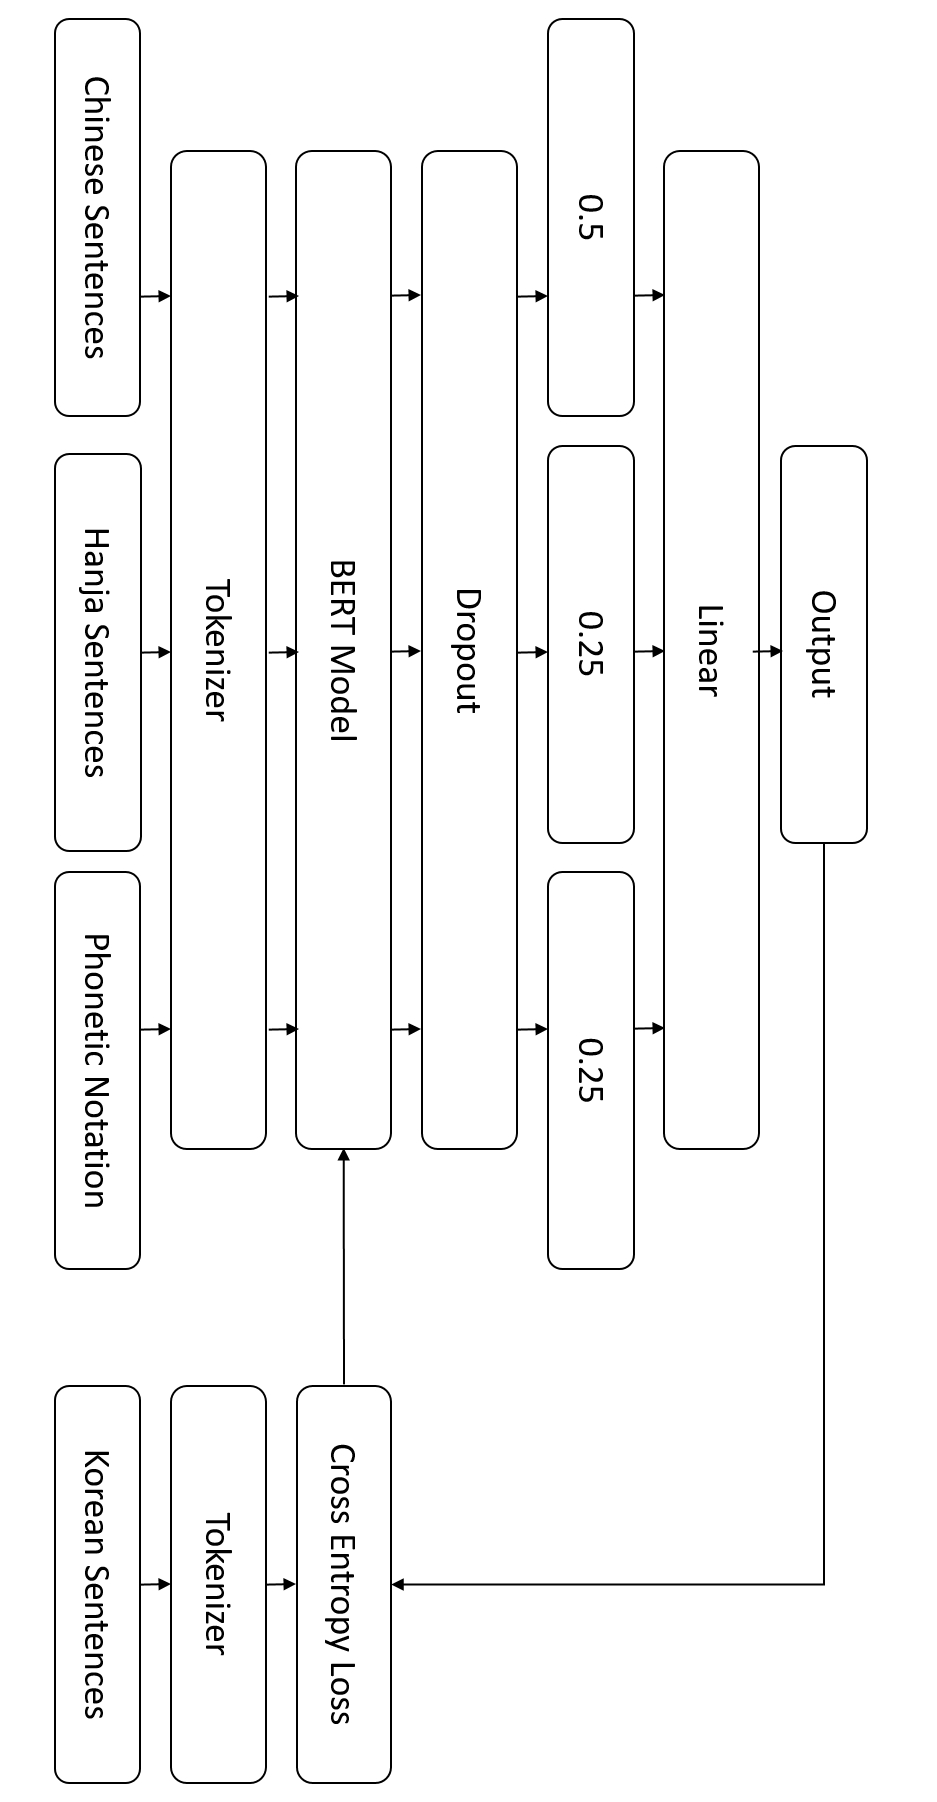
\includegraphics[width=0.75\linewidth]{fig_3_framework.jpg}
  \captionsetup{type=figure}
  \caption{Framework of model}
  \label{fig:framwork}
\end{figure}

%ch3.6.2
\subsection{Cross Entropy Loss}
To improve translation quality, we incorporate an entropy loss function \cite{zhang2018generalized}that encourages the model to produce diverse and accurate translations. The cross-entropy loss function used to train our model is defined as:

\[
\mathcal{L}_{\text{Cross\_Entropy\_Loss}}(p, \hat{p}) = -\sum_{i} p_i \log(\hat{p}_i)
\]

where $p$ is the true probability distribution (one-hot encoded), $\hat{p}$ is the predicted probability distribution (output of the neural network), and $i$ indexes the classes.

%ch4
\chapter{Experiment}
%ch4.1
\section{Dataset}
Our dataset comprises two primary sources. The first source involves 4937 transcripts obtained from the TED Talks website\cite{tedTalks}using a web crawler. Through alignment techniques, we retained a total of 182,750 aligned sentence pairs. The second source is the TED2020 dataset\cite{reimers-2020-multilingual-sentence-bert} sourced from the OPUS website, encompassing nearly 4,000 transcripts from TED and TEDx events since July 2020. For our study, we selected the Korean-Chinese (Taiwan) parallel corpus, yielding a substantial dataset of 3,189,220 aligned sentence pairs.

Tables 4.1 and 4.2 present the distribution of sentence pairs from TED Talks and TED2020 for both training and testing datasets.

%tab4.1

\begin{table}
\begin{tabularx}{0.9\linewidth}{p{3cm} p{3cm} p{3cm} p{3cm}}
Our Collection & Transcripts & Sentences & Proportion\\
\toprule
Train &  3949 & 146661 & 80\\[.3ex]
Test  &   988 & 36089 & 20 \\[.3ex]
\toprule
Total  &  4937 & 182750 & 100\\
\bottomrule
\end{tabularx}
\caption{TED Talks datasets}
\label{tab:notation}
\end{table}

%tab4.2
\begin{table}
\begin{tabularx}{0.9\linewidth}{p{4cm} p{4cm} p{4cm}}
Our Collection & Sentences & Proportion\\
\toprule
Train & 311376 & 80\\[.3ex]
Test & 77844 & 20 \\[.3ex]
\toprule
Total  & 3189220 & 100\\
\bottomrule
\end{tabularx}
\caption{TED2020 datasets}
\label{tab:notation}
\end{table}


%ch4.2
\section{BLEU Score}
In this paper, we utilize the BLEU (Bilingual Evaluation Understudy) score\cite{papineni-etal-2002-bleu} to evaluate the performance of our model. The BLEU score is a metric ranging from 0 to 100 that quantifies the similarity between machine-translated sentences and high-quality reference translations. A BLEU score of 0 indicates no overlap between the machine-translated sentence and the reference translation, while a score of 100 signifies perfect equivalence between the two. This metric is widely used in the field of machine translation to assess the accuracy and fluency of translated text by comparing n-grams of the candidate translation to those of the reference translation.

%ch4.3
\section{Result}
We first examine the losses and BLEU scores evaluated using our method with different tokenizers and Google Translation on our TED dataset. In Table 4.3, we compare the BLEU scores generated by Google Translation, Method 1, and Method 2. The results labeled as Google Translation were produced using the Google Translate service.

In Method 1, we use the BERT-base-Chinese tokenizer to generate embeddings of the input Chinese sentences during encoding. For decoding, we utilize the kim/bert-kor-base tokenizer to generate the output Korean sentences. Additionally, we use ckiplab/bert-base-chinese as our initial BERT model.

In Method 2, we enhance the BERT-base-Chinese tokenizer by incorporating Korean and Bopomofo tokens during both encoding and decoding stages. This approach leverages the additional linguistic information provided by these tokens to improve translation quality. Similar to Method 1, we use ckiplab/bert-base-chinese as our initial BERT model.

%table 4.3
\begin{table}
\begin{tabularx}{0.9\linewidth}{p{3cm} p{2cm} p{4cm} p{4cm}}
Method & Gooletrans & Our Method 1 & Our Method 2\\
\toprule
Tokenizer &  - & Src: Bert-base-Chinese 
 & Bert-base-Chinese\\
&& Tgt: Kim/bert-kor-base & (Add korean and Bopomofo tokens)
\\[.3ex]
\\
Model  &   - & ckiplab/bert-base-chinese+linear & ckiplab/bert-base-chinese+linear
 \\[.3ex]
\toprule
BLEU score  &  25.32 & 16.57 & \textbf{25.77}\\
\bottomrule
\end{tabularx}
\caption{BLUE scores of Our Methods}
\label{tab:notation}
\end{table}

Next, we compare the results generated by our method using joint embeddings with different proportions and datasets. Our comparison includes four scenarios: 'only Chinese', 'Chinese + Hanja', 'Chinese + Bopomofo', and 'Chinese + Hanja + Bopomofo'.

Figure 4.1 shows the training loss and testing loss histories for the four cases trained on our TED dataset. Figure 4.2 presents the training loss and testing loss histories for the same four cases trained on the TED2020 dataset.

Although losses do not directly correlate with BLEU scores, we observe lower losses in cases utilizing Hanja embeddings and higher losses in cases using only Chinese and Bopomofo embeddings. Specifically, the model using Chinese and Bopomofo embeddings exhibits the highest loss, likely due to the Bopomofo tokens not being pre-trained in the BERT-base-Chinese tokenizer.

% figure 4.1
\begin{figure}[h!]
  \centering
  \subfloat[Train Loss]{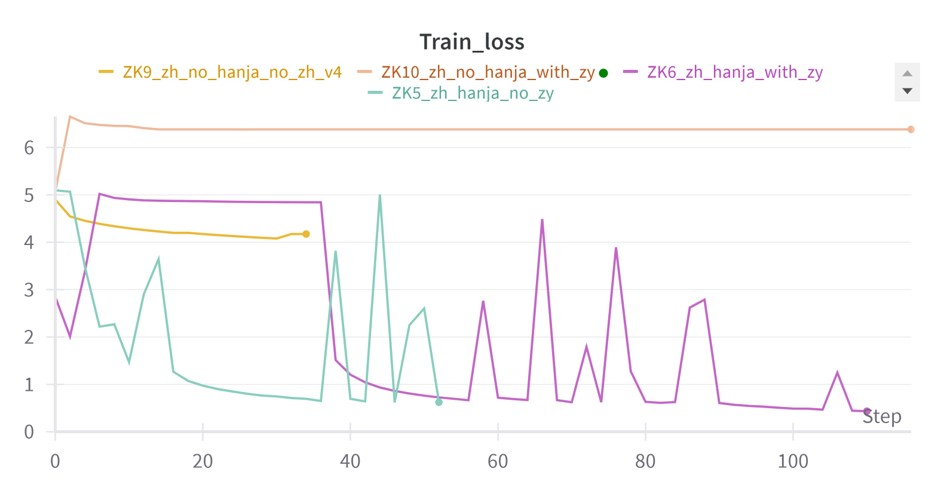
\includegraphics[width=0.49\textwidth]{fig_5_1_1.jpg}\label{fig_5_1_1.jpg}}
  \hfill
  \subfloat[Test Loss]{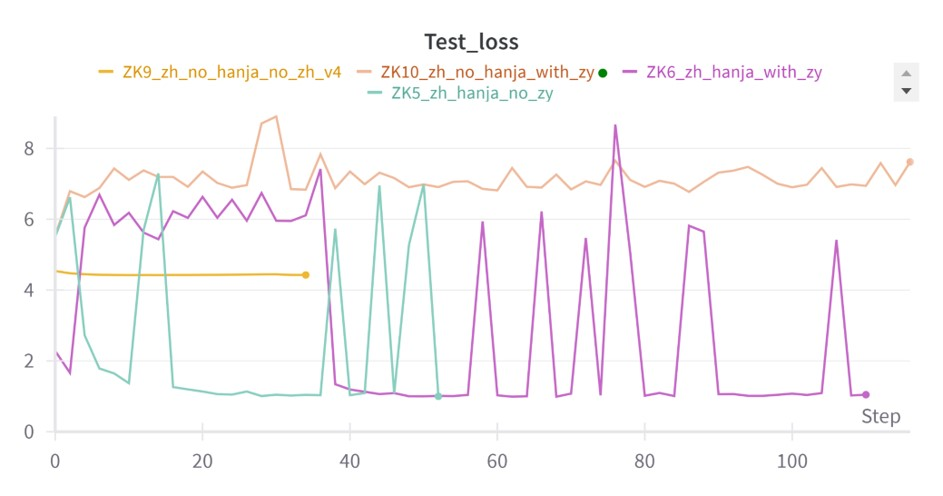
\includegraphics[width=0.49\textwidth]{fig_5_1_2.jpg}\label{fig_5_1_2.jpg}}
  \captionsetup{type=figure}
  \caption{Train and Test Loss of Our Method in Ted Talks Dataset}
  \label{fig:naver dictionary}
\end{figure}

%figure 4.2
\begin{figure}[h!]
  \centering
  \subfloat[Train Loss]{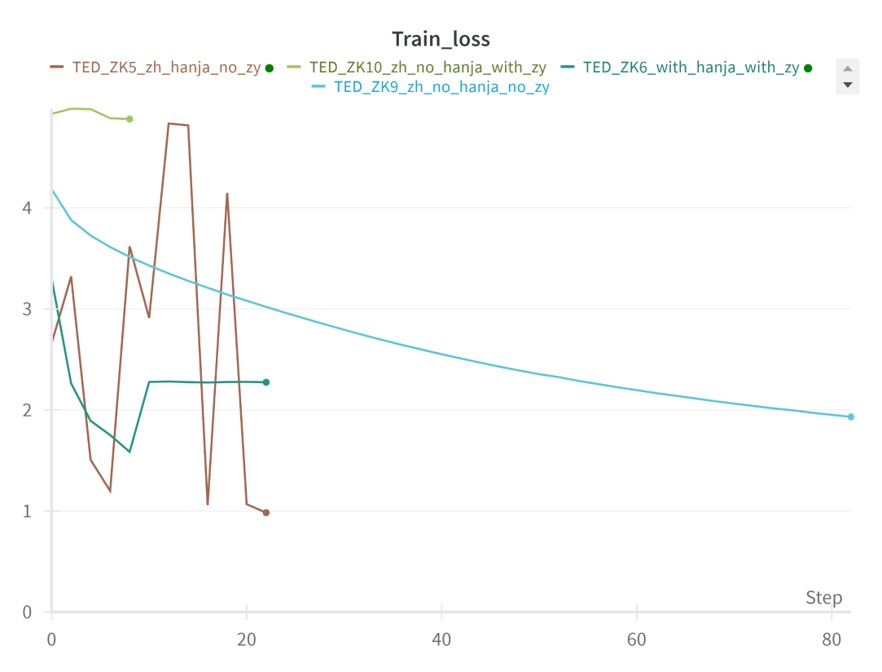
\includegraphics[width=0.49\textwidth]{fig_5_2_1.jpg}\label{fig_5_2_1.jpg}}
  \hfill
  \subfloat[Test Loss]{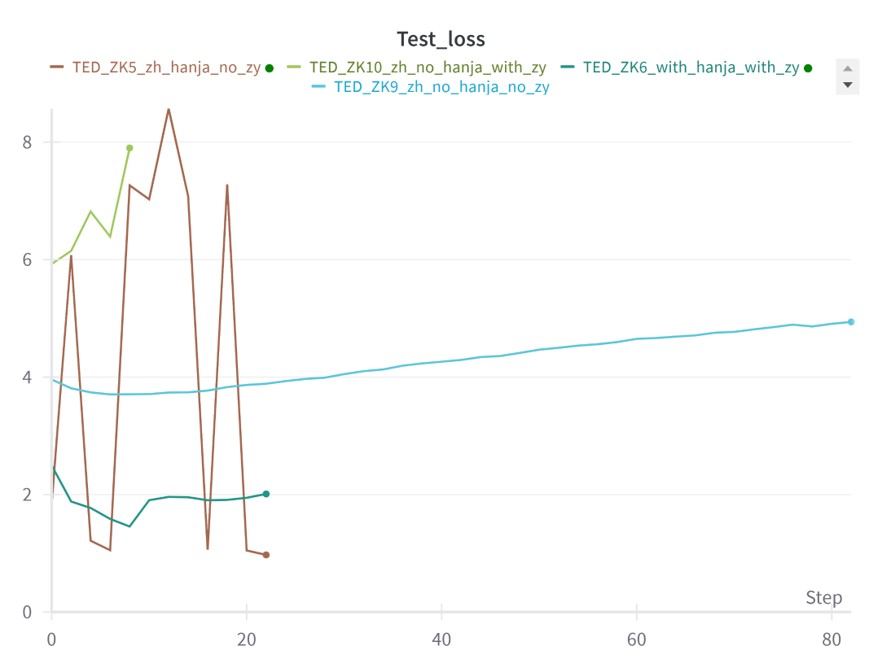
\includegraphics[width=0.49\textwidth]{fig_5_2_2.jpg}\label{fig_5_2_2.jpg}}
  \captionsetup{type=figure}
  \caption{Train and Test Loss of Our Method in Ted2020 Dataset}
  \label{fig:naver dictionary}
\end{figure}

Table 4.4 shows the BLEU scores evaluated for the four cases trained on our TED dataset. Table 4.5 presents the BLEU scores evaluated for the same four cases trained on the TED2020 dataset.

We use a 0.5:0.5 proportion for both 'Chinese + Hanja' and 'Chinese + Bopomofo' embeddings and a 0.5:0.25:0.25 proportion for our joint embedding 'Chinese + Hanja + Bopomofo'.

In Table 4.4, the best BLEU score of 25.77 is achieved using the 'Chinese + Hanja + Bopomofo' embedding, with only a slight difference from the score obtained using the 'Chinese + Hanja' embedding. Conversely, the 'only Chinese' embedding results in a BLEU score of 1.13, and the 'Chinese + Bopomofo' embedding yields a score of 0.01.

In Table 4.5, the highest BLEU score of 15.33 is achieved using the 'Chinese + Hanja' embedding. The 'Chinese + Hanja + Bopomofo' embedding scores 7.86. In contrast, the 'only Chinese' embedding results in a BLEU score of 1.36, while the 'Chinese + Bopomofo' embedding scores 0.00.

The lower performance of models using Bopomofo tokens is likely due to the lack of pre-training for these tokens in the BERT-base-Chinese tokenizer and the initial 'ckiplab/bert-base-chinese' BERT model. This makes it more challenging to generate complete Korean sentences when training only on Chinese and Bopomofo sentences.

% table 4.4
\begin{table}
\begin{tabularx}{0.9\linewidth}{p{4cm} p{2cm} p{2cm} p{2cm} p{2cm}}
Enbedding & & Propotion & &\\
\toprule
Zh-tw &  1 & 0.5 & 0.5 & 0.5 \\
Hanja  &   0 & 0.5 & 0 & 0.25\\[.3ex]
Bopomofo  &  0 & 0 & 0.5 & 0.25\\
\toprule
BLEU score  &  1.13 & 25.36 & 0.01 & \textbf{25.77}\\
\bottomrule
\end{tabularx}
\caption{BLUE scores of Our Methods in TED Talks dataset}
\label{tab:notation}
\end{table}

% table 4.5
\begin{table}
\begin{tabularx}{0.9\linewidth}{p{4cm} p{2cm} p{2cm} p{2cm} p{2cm}}
Enbedding & & Propotion & &\\
\toprule
Zh-tw &  1 & 0.5 & 0.5 & 0.5 \\
Hanja  &   0 & 0.5 & 0 & 0.25\\[.3ex]
Bopomofo  &  0 & 0 & 0.5 & 0.25\\
\toprule
BLEU score  &  1.36 & \textbf{15.33} & 0.00 & 7.86\\
\bottomrule
\end{tabularx}
\caption{BLUE scores of Our Methods in TED2020 dataset}
\label{tab:notation}
\end{table}



%ch5
\chapter{Discussion}
In this section, we will examine the translations generated by Google Translate, our Method 1, and our Method 2. Additionally, we will utilize PCA (Principal Component Analysis)\cite{MACKIEWICZ1993303} and t-SNE (t-distributed Stochastic Neighbor Embedding)\cite{tsne} methods to perform dimensionality reduction and visualize the embeddings generated by the initial BERT model and the BERT model from our approach. We will compare the differences in embedding distributions across "Chinese," "Hanja," "Bopomofo," "joint embedding," and "Korean" embeddings.

%ch5.1
\section{Case Study}
First, we compare the translations generated by Google Translate with those from our Method 1. 

Table 5.1 compares the translations generated by Google Translate and our Method 1.

In Case 1, the BLEU scores for both translations are low. Google Translate produces a coherent and grammatically correct sentence, capturing the overall structure of the sentence and maintaining readability. However, the translation deviates from the original meaning by introducing concepts like "not paying attention," which are not present in the reference. The result from Google Translate is not ideal due to the difference in expression between the source and target sentences. The meaning "I'm the only one not paying attention" in the Chinese source translates to "Everyone is paying attention except me" in the Korean reference, failing to accurately convey the specific context of the reference sentence.

As for our method, while the example output is fragmented, it demonstrates that the model is attempting to capture specific tokens and structures from the source. This indicates potential for improvement in handling complex sentence structures and maintaining original meanings. However, the current output is incoherent and fails to produce a readable sentence. It struggles with tokenization and syntax, resulting in a nonsensical translation. Despite these shortcomings, further refinement could lead to significant improvements in translation accuracy.

In case 2, Google Translate has a lower BLEU score, our method demonstrates several advantages over Google Translate in this case.

Firstly, our method preserves the overall structure and context of the reference sentence much more accurately. It correctly translates \krtext{"그려진 지 500년이 훌쩍 넘고" and "눈썹도 사라진 지 한참 지나서,"} which closely matches the original meaning. Google Translate, on the other hand, introduces inaccuracies by translating the phrase into \krtext{"그것은 500 년이 지난 후에 만들어졌습니다 - 예수와 속눈썹은 오랫동안 사라졌습니다,"} which deviates significantly from the original context.

Secondly, our method correctly maintains the specific mention of the "Mona Lisa" and the protective "bulletproof frame" against earthquakes. Google Translate's version, \krtext{"방탄과 지진의 유리 상자에서 보호되었습니다,"} introduces confusion by combining elements incorrectly and introducing the term "glass box," which is not present in the reference.

While our method does have repetition in the phrase \krtext{"이겨 이겨 내는,"} it still retains the key elements and context of the original sentence more faithfully. This indicates that our model captures specific tokens and structure from the source, showing potential for further improvement in maintaining accuracy and coherence.

% table 5.1
\begin{figure}[h!]
  \centering
  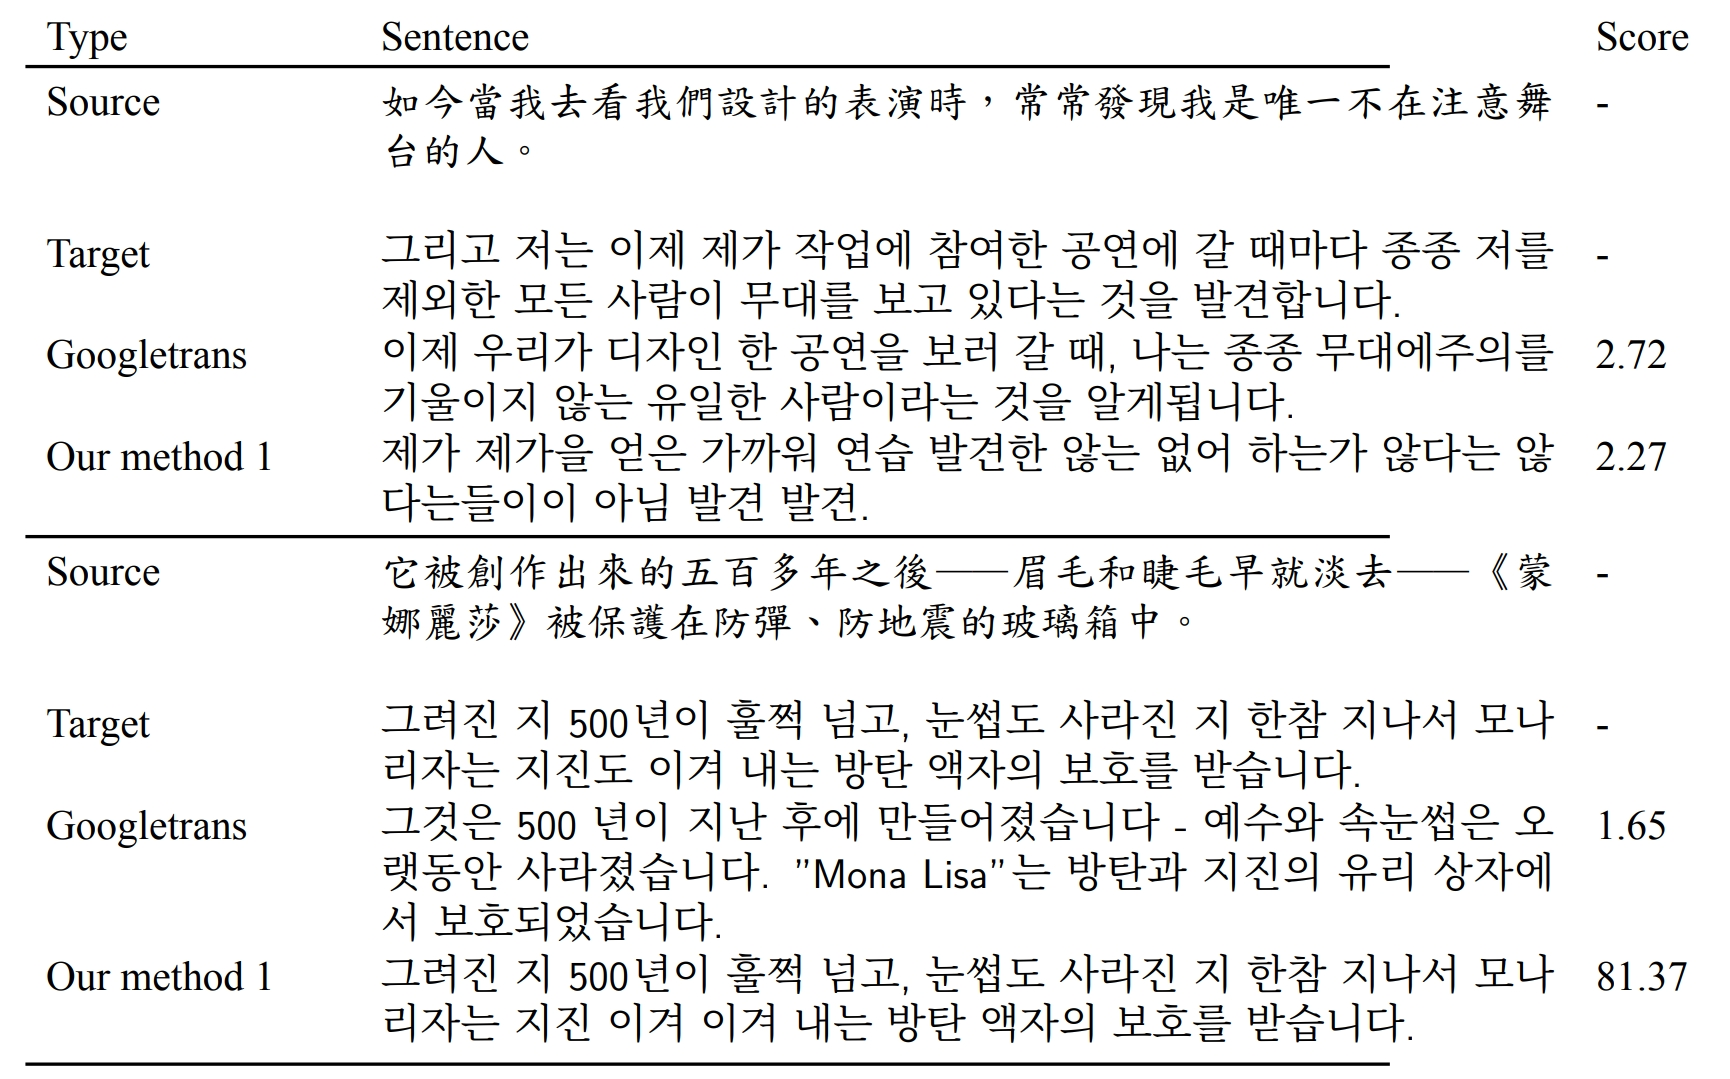
\includegraphics[width=\linewidth]{tab_5_1.jpg}
  \captionsetup{type=table}
  \caption{Case Study - Googletrans and Our Method 1}
  \label{tab:Case Study - Googletrans and Our Method 1}
\end{figure}

%\begin{table}
%\begin{tabularx}{0.9\linewidth}{p{3cm} p{12cm} p{3cm}}
%Type & Sentence & Score\\
%\toprule
%Source
%&如今當我去看我們設計的表演時,常常發現我是唯一不在注意舞台的人。 
%& -\\
%\\
%Target
%&\krtext{그리고 저는 이제 제가 작업에 참여한 공연에 갈 때마다 종종 저를 제외한 모든 사람이 무대를 보고 있다는 것을 발견합니다.}
%& -\\
%Googletrans
%&\krtext{이제 우리가 디자인 한 공연을 보러 갈 때, 나는 종종 무대에주의를 기울이지 않는 유일한 사람이라는 것을 알게됩니다.}
%& 2.72 \\ 
 %Our method 1
% &\krtext{제가 제가을 얻은 가까워 연습 발견한 않는 없어 하는가 않다는 않다는들이이 아님 발견 발견.}
% & 2.27\\
%\toprule
%Source
%&它被創作出來的五百多年之後——眉毛和睫毛早就淡去——《蒙娜麗莎》被保護在防彈、防地震的玻璃箱中。
%& -\\
%\\
%Target
%&\krtext{그려진 지 500년이 훌쩍 넘고, 눈썹도 사라진 지 한참 지나서 모나리자는 지진도 이겨 내는 방탄 액자의 보호를 받습니다.}
%& -\\
%Googletrans
%&\krtext{그것은 500 년이 지난 후에 만들어졌습니다 - 예수와 속눈썹은 오랫동안 사라졌습니다. "Mona Lisa"는 방탄과 지진의 유리 상자에서 보호되었습니다.}
%& 1.65 \\ 
% Our method 1
% &\krtext{그려진 지 500년이 훌쩍 넘고, 눈썹도 사라진 지 한참 지나서 모나리자는 지진 이겨 이겨 내는 방탄 액자의 보호를 받습니다.}
% & 81.37\\
%\bottomrule
%\end{tabularx}
%\caption{Case Study - Googletrans and Our Method 1}
%\label{tab:notation}
%\end{table}

Next, we examine the translations produced by our Method 2 across the four cases. 

Table 5.2 compares the translations generated by our Method 2 using different embedding proportions.

In all cases, the BLEU scores are low across all methods. For the model that uses only Chinese embeddings, it almost always generates short, fragmentary sentences, often composed of irrelevant words. The model that uses Chinese and Bopomofo embeddings produces slightly longer sentences, but they tend to contain repeated words, resulting in incomplete and illogical sentences. The model that employs Chinese and Hanja embeddings shows highly variable quality; it performs better with short sentences but generates long, incorrect sentences for longer input.

For the model using joint embeddings, although the BLEU scores are still not high, the translations are generally more similar to the reference sentences than those produced by other methods. In some cases, it even outperforms Google Translate. This suggests that the joint embedding approach, despite its low scores, captures more accurate translations and better maintains the context of the original sentences.

In Case 1, the joint embedding model correctly generated \krtext{"노란색"} (yellow) and \krtext{"아직 잘 모릅니다"} (still don't know well). In contrast, Google Translate also correctly generated \krtext{"노란색"} (yellow) and \krtext{"모릅니다"} (don't know), but it omitted \krtext{"아직"} (still) and added an extra \krtext{"우리"} (we). Additionally, Method 1 incorrectly translated "黃色的" (yellow) as \krtext{"파란 흰색 색"} (blue, white) and included the word \krtext{"아름답"} (beautiful), which is not present in the reference sentence.

In Case 2, the joint embedding model correctly generated \krtext{"밤에"} (at night), \krtext{"잠"} (sleep), and \krtext{"잘 수 없었습니다"} (could not sleep). In contrast, Google Translate also correctly generated \krtext{"밤에"} (at night), \krtext{"잠을"} (sleep), and \krtext{"잘 수 없었다"} (could not sleep), but it incorrectly used honorific endings. Additionally, Method 1 correctly generated \krtext{"밤에"} and \krtext{"잠을."} However, this sentence is a negative statement, but Method 1 mistakenly translates it into an affirmative statement.

In Case 3, the joint embedding model correctly generated \krtext{"저는" }(I), \krtext{"여성들"} (women), \krtext{"함께"} (together), \krtext{"51 펀드"} (51 fund), and \krtext{"있습니다"} (have). In contrast, Google Translate also correctly generated \krtext{"여성들"}, \krtext{"51 펀드"}, and \krtext{"습니다"}. However, it mistranslated "現在" (now) as \krtext{"이제"} (now) instead of \krtext{"지금" }(now), despite their similar meanings. Additionally, Method 1 only correctly generated \krtext{"지금"} (now) and \krtext{"여성들"} (women); other words were mostly incorrect.

% table 5.2
\begin{table}
\begin{tabularx}{0.9\linewidth}{p{3cm} p{12cm} p{3cm}}
Type & Sentence & Score\\
\toprule
% case1
Source
&我們還不清楚黃色的是什麼。
& -\\
\\
Target
&\krtext{노란색은 아직 잘 모릅니다.}
& -\\
Googletrans
&\krtext{우리는 노란색이 무엇인지 모릅니다.}
& 21.36 \\ 
 Our method 1
 &\krtext{파란 흰색 색 아름답 전혀 알 알지.}
 & 5.52\\
Our method 2\\
Only Chinese
&\krtext{케이, 꽊?}
& 0.00 \\ 
Chinese+Bopomofo
&\krtext{검색 났 났 쵳 이렇듯 이렇듯 났 이렇듯 이렇듯 이렇듯 이렇듯.}
& 3.39 \\ 
Chinese+Hanja
&\krtext{무가 아니죠 잘 모릅니다.}
& 20.56 \\ 
 Joint
 &\krtext{노란색플로 아직 잘 모릅니다.}
 & 66.87\\
 % case2
\toprule
Source
&我晚上睡不著覺。
& -\\
\\
Target
&\krtext{밤에 잠을 잘 수 없었습니다.}
& -\\
Googletrans
&\krtext{나는 밤에 잠을 잘 수 없었다.}
& 43.47 \\ 
 Our method 1
 &\krtext{저 밤에 잠을 잠을 입고.}
 & 14.54\\
Our method 2\\
Only Chinese
&\krtext{슽먋인가봐요.}
& 0.00 \\ 
Chinese+Bopomofo
&\krtext{몹 면으로 쏸 이렇듯 이렇듯 이렇듯.}
& 6.567 \\ 
Chinese+Hanja
&\krtext{거절 챪 비자 잘 최상급 최상급.}
& 7.81 \\ 
 Joint
 &\krtext{밤에 잠 겮 잘 수 없었습니다.}
 & 43.47\\
% case 3
\toprule
Source
&現在,和一些很棒的女性合作,我要發起「51基金」。
& -\\
\\
Target
&\krtext{지금 저는 몇 명의 대단한 여성들과 함께, "51 펀드" 라는 것을 론 칭하고 있습니다.}
& -\\
Googletrans
&\krtext{이제 위대한 여성들과 협력하여 "51 펀드"를 시작하고 싶습니다.}
& 14.23 \\ 
 Our method 1
 &\krtext{지금 훌륭한 훌륭한 는 나은 여성들이 저는 저는 800란.}
 & 2.61\\
Our method 2\\
Only Chinese
&\krtext{이면 슽 ),}
& 0.48 \\ 
Chinese+Bopomofo
&\krtext{검색 검색,즙은즙은 네티즌......,. 이렇듯.}
& 2.56 \\ 
Chinese+Hanja
&\krtext{몸에팀의 퇴직 수고붚 먹고있어요 눈에는 눈에는,, 13 42 " " 났어요 났어요 사장이 어려워서뉴얼.}
& 2.23 \\ 
 Joint
 &\krtext{툣 저는 정성이작을쉕 부모의돉 여성 들아요 함께, " 51 펀드 " 라는 것 겮굪 칭쒰 있습니다.}
 & 37.16\\
 
\bottomrule
\end{tabularx}
\caption{Case Study - Embeddings in four cases}
\label{tab:notation}
\end{table}

Finally, we analyze the results from our best model using Hanja sentences to understand the relationship between the number of generated Hanja characters in a sentence and the corresponding BLEU score.

Table 5.3 illustrates that sentences containing more Hanja characters tend to introduce more translation errors. This is because the joint embedding model may deviate further from the Korean embedding space, impacting translation accuracy.

In Case 1, seven Hanja words were identified in the Korean sentence: \krtext{"미국"}-"美國" (America), \krtext{"백인 남자"}-"伯仁" (white man), \krtext{"폭력"}-"暴力" (violence), \krtext{"정신"}-"精神" (mental), \krtext{"질환"}-"疾患" (disease), \krtext{"주차"}-"駐車" (parking), and \krtext{"분쟁"}-"紛爭" (dispute). However, none of these words appeared in the translation.

In Case 2, only one Hanja word, \krtext{"학교"}-"學校" (school), was found in the Korean sentence. The translation correctly rendered the text before \krtext{"학교"} but contained errors after this word in the sentence.

%table 5.3
\begin{figure}[h!]
  \centering
  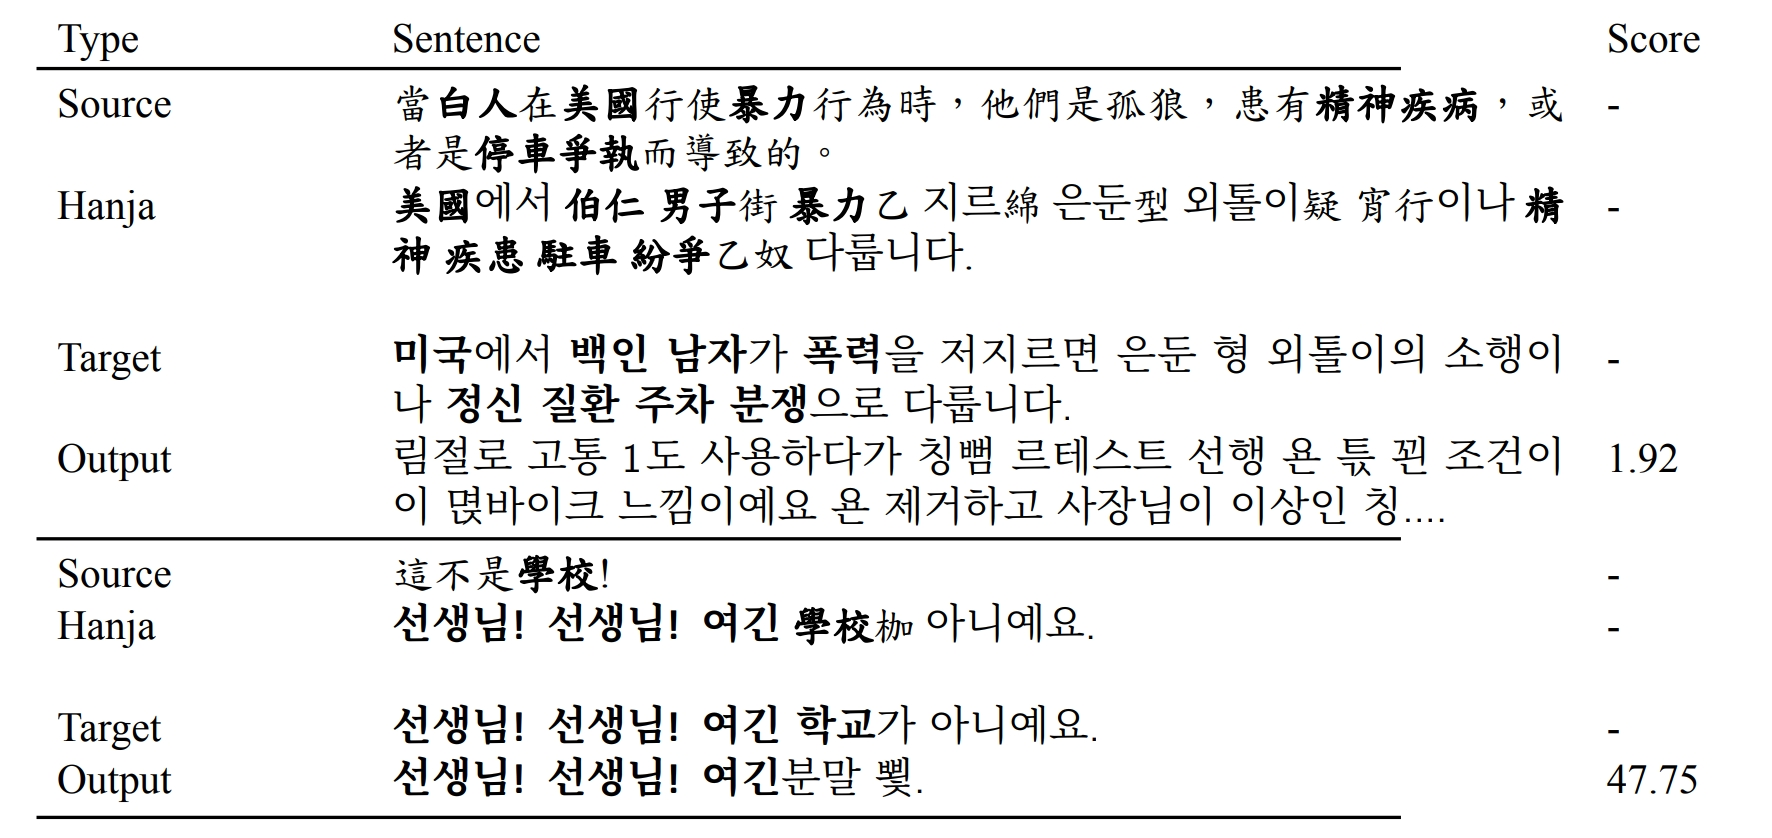
\includegraphics[width=\linewidth]{tab_5_3.jpg}
  \captionsetup{type=table}
  \caption{Case Study - Examine Hanja Sentence}
  \label{tab:Case Study - Examine Hanja Sentence}
\end{figure}

%\begin{table}
%\begin{tabularx}{0.9\linewidth}{p{3cm} p{12cm} p{3cm}}
%Type & Sentence & Score\\
%\toprule
%Source
%&當\textbf{白人}在\textbf{美國}行使\textbf{暴力}行為時,他們是孤狼,患有\textbf{精神疾病},或者是\textbf{停車爭執}而導致的。
%& -\\
%Hanja
%&\textbf{美國}\krtext{에서} \textbf{伯仁 男子}街 \textbf{暴力}乙 \krtext{지르}綿 \krtext{은둔} 型 \krtext{외톨이}疑 宵行\krtext{이나} \textbf{精神 疾患 駐車 紛爭}乙奴 \krtext{다룹니다}. 
%& -\\
%\\
%Target
%&\krtext{\textbf{미국}에서 \textbf{백인 남자}가 \textbf{폭력}을 저지르면 은둔 형 외톨이의 소행이나 \textbf{정신 질환 주차 분쟁}으로 다룹니다.} 
%& -\\
%Output
%&\krtext{림절로 고통 1도 사용하다가 칭뻠 르테스트 선행 욘 튻 꾄 조건이 이 멵바이크 느낌이예요 욘 제거하고 사장님이 이상인 칭....}
%& 1.92 \\ 
%\toprule
%Source
%&這不是\textbf{學校}!
%& -\\
%Hanja
%&\krtext{\textbf{선생님! 선생님! 여긴}} \textbf{學校}枷 \krtext{아니예요.}
%& - \\
%\\
%Target
%&\krtext{\textbf{선생님! 선생님! 여긴 학교}가 아니예요.}
%& -\\
%Output
%&\krtext{\textbf{선생님! 선생님! 여긴}분말 뾫.}
%& 47.75 \\
%\bottomrule
%\end{tabularx}
%\caption{Case Study - Examine Hanja Sentence}
%\label{tab:notation}
%\end{table}


%ch5.2
\section{Embedding Analysis}
We perform an embedding analysis using PCA and t-SNE on the original CKIP BERT model and our enhanced BERT model. This analysis aims to visualize and compare the embedding distributions produced by both models, highlighting the improvements and differences introduced by our modifications.

%5.2.1
\subsection{Principal Component Analysis}
PCA primarily achieves three effects: Dimensionality Reduction, Orthogonal Transformation, and Eigenvalues and Eigenvectors.

\textbf{Dimensionality Reduction:} PCA is primarily used to reduce the dimensionality of large datasets while retaining as much variability (information) as possible. It achieves this by transforming the data into a new set of orthogonal (uncorrelated) variables called principal components, which are ordered by the amount of variance they capture from the data.

\textbf{Orthogonal Transformation:} PCA performs an orthogonal transformation to convert the original set of possibly correlated variables into a set of linearly uncorrelated variables. These new variables, the principal components, are derived such that the first principal component captures the most variance in the data, and each subsequent component captures the remaining variance under the constraint that it is orthogonal to the preceding components.

\textbf{Eigenvalues and Eigenvectors:} The core of PCA involves computing the eigenvalues and eigenvectors of the covariance matrix of the data. The eigenvectors determine the direction of the principal components (the axes of the new feature space), and the eigenvalues determine their magnitude (the importance or variance captured by each component). By selecting the top k eigenvectors corresponding to the largest eigenvalues, we can project the data onto a k-dimensional subspace, thereby reducing the dimensionality.

In Figure 5.1, we perform an embedding analysis using PCA on the original CKIP BERT model and our enhanced BERT model. We show the distribution of embeddings for five cases: 'Chinese', 'Korean', 'Hanja', 'Bopomofo', and 'Joint Embedding'. We randomly selected 200 sentences in each case to illustrate their embedding distribution. Figure 5.1(a) presents the embeddings from the original CKIP BERT model, while Figure 5.1(b) presents the embeddings from our enhanced BERT model.

In Figure 5.1(a), the distance between 'Korean' and 'Bopomofo' embeddings is closer than that to the 'Chinese' embeddings because 'Korean' and 'Bopomofo' were not trained on the original CKIP BERT model. Consequently, the embeddings for 'Korean' and 'Bopomofo' are in their initial state for the original CKIP BERT model. The 'Hanja' embeddings are scattered, and the 'Joint Embedding' is positioned between the 'Chinese', 'Hanja', and 'Bopomofo' embeddings.

On the other hand, in Figure 5.1(b), the embeddings for 'Korean' and 'Hanja' are closer, indicating that they are derived from the same language family. Similarly, the embeddings for 'Chinese' and 'Bopomofo' are closer to each other than to other embeddings, distinguishing them as part of a different language group from 'Korean' and 'Hanja'. This visualization highlights the improvements and distinctions introduced by our modifications to the BERT model.

%figure 5.1
\begin{figure}[h!]
  \centering
  \subfloat[Initial BERT model]{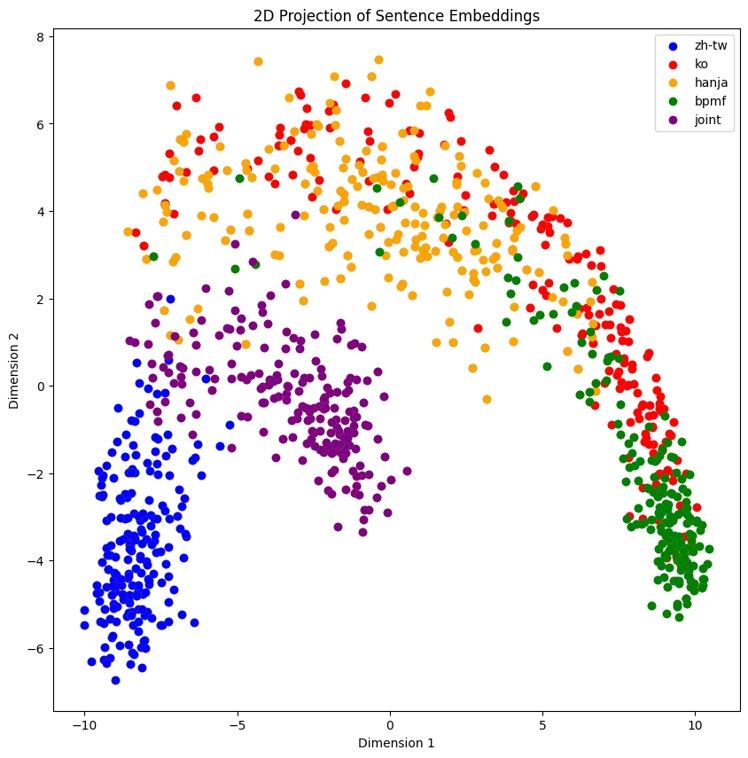
\includegraphics[width=0.49\textwidth]{fig_ori_pca.jpg}\label{fig_ori_pca.jpg}}
  \hfill
  \subfloat[Our model]{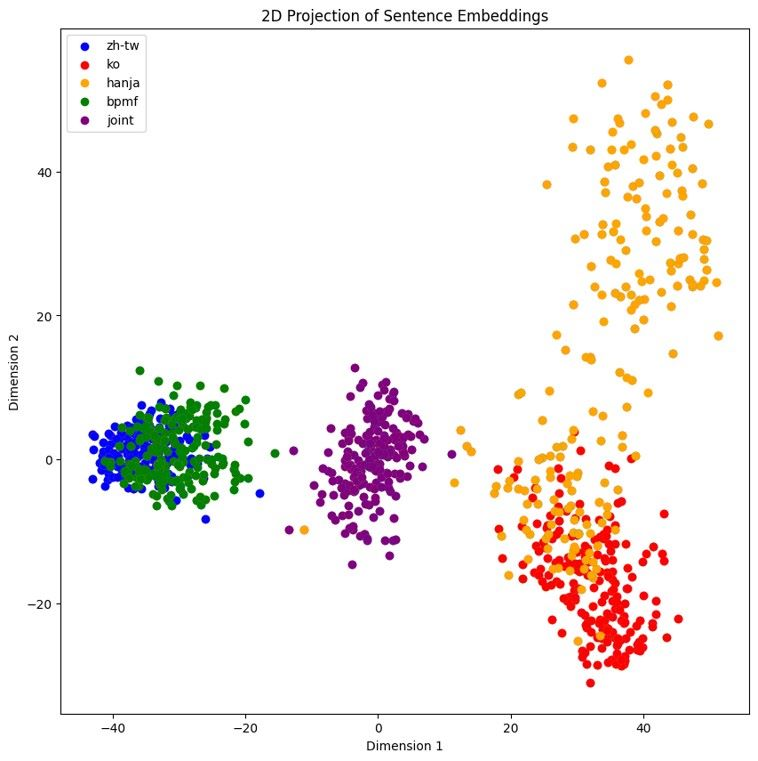
\includegraphics[width=0.49\textwidth]{fig_my_pca.jpg}\label{fig_my_pca.jpg}}
  \captionsetup{type=figure}
  \caption{Embedding analyzation with PCA of the original CKIP BERT model and our BERT model}
  \label{fig:naver dictionary}
\end{figure}

%5.2.2
\subsection{t-Distributed Stochastic Neighbor Embedding}
t-SNE primarily offers three advantages: Non-Linear Dimensionality Reduction, Probability Distributions, and Preserving Local Structure.

\textbf{Non-Linear Dimensionality Reduction:} Unlike PCA, t-SNE is a non-linear dimensionality reduction technique primarily used for data visualization. It is especially effective at embedding high-dimensional data into two or three dimensions for visualization purposes, while preserving the local structure (neighborhood relationships) of the data points.

\textbf{Probability Distributions:} t-SNE converts the high-dimensional Euclidean distances between data points into conditional probabilities that represent similarities. It then aims to match these similarities in a lower-dimensional space. The method minimizes the Kullback-Leibler (KL) divergence between the probability distributions of the original high-dimensional data and the lower-dimensional embedding. This optimization process ensures that similar points in high-dimensional space remain close in the lower-dimensional representation.

\textbf{Preserving Local Structure:} While PCA focuses on maximizing variance and maintaining global structure, t-SNE is designed to preserve the local structure of the data. This means it excels at keeping close points together in the embedding space, making it particularly useful for visualizing clusters or groups in the data. However, t-SNE might distort the global relationships between clusters, which is a trade-off for its effectiveness in highlighting local structures.

In Figure 5.2, we perform an embedding analysis using t-SNE on the original CKIP BERT model and our enhanced BERT model. Similar to Figure 5.1, we show the distribution of embeddings for five cases: 'Chinese', 'Korean', 'Hanja', 'Bopomofo', and 'Joint Embedding'. We randomly selected 200 sentences in each case to illustrate their embedding distribution. Figure 5.2(a) presents the embeddings from the original CKIP BERT model, while Figure 5.2(b) presents the embeddings from our enhanced BERT model.

The results are consistent with those shown in Figure 5.1. In Figure 5.2(b), the embedding distribution indicates that 'Chinese' and 'Bopomofo' belong to one language group, while 'Korean' and 'Hanja' belong to another. This visualization highlights the improvements and distinctions introduced by our modifications to the BERT model.

% figure 5.2
\begin{figure}[h!]
  \centering
  \subfloat[Initial BERT model]{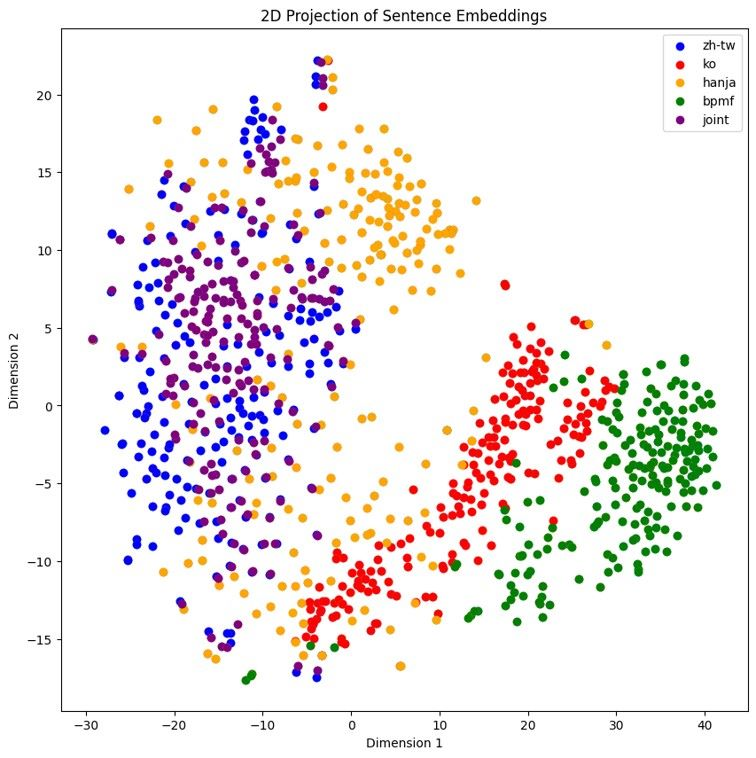
\includegraphics[width=0.49\textwidth]{fig_ori_tsne.jpg}\label{fig_ori_tsne.jpg}}
  \hfill
  \subfloat[Our model]{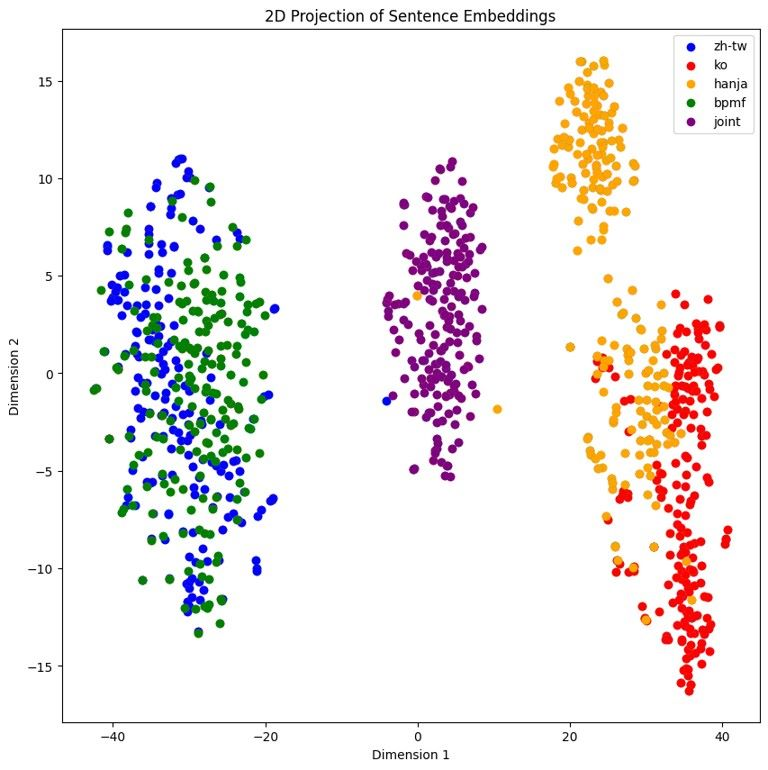
\includegraphics[width=0.49\textwidth]{fig_my_tsne.jpg}\label{fig_my_tsne.jpg}}
  \captionsetup{type=figure}
  \caption{Embedding analyzation with tSNE of the original CKIP BERT model and our BERT model}
  \label{fig:naver dictionary}
\end{figure}

%ch6
\chapter{Conclusions and Future Work}
%ch6.1
\section{Conclusions}
In this paper, our objective is to improve an NMT model for translating between Traditional Chinese and Korean by integrating Hanja and Bopomofo embeddings. We assess our model using the BLEU score, and the results in Section 4.3 demonstrate that our method outperforms Google Translate on the TED Talks dataset. Additionally, we experiment with different proportions of 'Chinese', 'Hanja', and 'Bopomofo' embeddings, finding that performance improves when Hanja embeddings are included. This experiments show that the integration of Hanja embeddings significantly enhances translation quality, highlighting the importance of incorporating linguistic elements native to the target language.

In the case study, we examine translation cases for Google Translate, our Method 1, and four embedding proportions in our Method 2. To validate the effectiveness of our approach, we visualize the embeddings' distribution. Using both PCA and t-SNE for dimensionality reduction, we observe that the BERT model, after training, is more effective in distinguishing the differences between Traditional Chinese and Korean, thus ensuring more accurate translations.

In Section 5.1, we analyze the relationship between the number of generated Hanja in the sentences and our output translations. Contrary to our expectations, a higher number of generated Hanja in the sentence resulted in poorer translation quality, likely due to the lack of Korean training for our BERT model. While the inclusion of Hanja shows promise, the quality of translations can diminish when there are too many Hanja characters due to insufficient training on the Korean language, indicating a need for further model refinement.

Moreover, we designed a method to align and obtain parallel corpora between Traditional Chinese and Korean from the TED websites. This approach helps in overcoming the challenge of limited parallel data, providing a foundation for future improvements in NMT systems between these languages.

%ch6.2
\section{Future Work}
In this paper, our model is straightforward: we use a BERT model to extract embeddings and a linear layer to transform them to the Korean domain. To enhance our model, we plan to use a transformer model as our main framework, incorporating our BERT model for embedding extraction.

To address the uncertainty of Bopomofo embeddings, we will utilize another pre-trained BERT model for Chinese phonetics, as proposed by Sun Zijun et al. in 2021.\cite{sun-etal-2021-chinesebert}

\newpage
\AddToContents{Bibliography}
\printbibliography

\end{document}
